% !TeX root=../../../main.tex

\chapter{روش‌های پیشین}
% دستور زیر باعث عدم‌نمایش شماره صفحه در اولین صفحهٔ این فصل می‌شود.
%\thispagestyle{empty}

\section{مقدمه}
در فصل گذشته به معرفی مفاهیم و موضوعات مرتبط با این حوزه پرداخته شد. در ادامه در این فصل با توجه به اطلاعاتی که کسب کرده‌اید به معرفی و بررسی روش‌هایی که مرتبط با موضوع این پایان‌نامه است پرداخته خواهد شد و نتایج آن‌ها را برای فرض‌های و داده‌های ورودی خود مشاهده خواهیم نمود. در این بین تا جایی که ممکن باشد به بررسی نقاط قوت و ضعف آن‌ها نیز خواهیم پرداخت و در انتهای این فصل یک جدول مقایسه بین روش‌هایی که تا به حال معرفی شده‌اند را ارائه خواهیم داد.

%در ابتدای این فصل به معرفی مقاله و روش SCITE خواهیم پرداخت که البته یکی از مقالات اصلی پایان‌نامه جاری می‌باشد و یکی از روش‌های پیشنهادی در فصل آینده نیز بر پایه همین روش می‌باشد.


%\section{\gls{tumorevolutionarytreeinference} با استفاده از داده‌های \gls{scs}}
%\gls{cancer} نامی است که به مجموعه‌ای از بیماری‌ها اطلاق می‌شود که از تکثیر مهار نشده سلول‌ها پدید می‌آیند. تحقیقات انجام شده نشان می‌دهد که سرطان در واقع یک فرآیند تکاملی از جهش‌های  ژنتیکی، شامل حذف و تغییر تعداد کپی ، حذف و تغییر تک نوکلئوتیدد‌ها  ، بازسازی و جایگزینی ژن‌ها در سلول‌های توموری است. در واقع تومور زمانی ایجاد می‌شود که یک سلول جهش یافته بتواند با عبور از سیستم دفاعی بدن زندگی کرده و تکثیر شود به گونه‌ای که نسبت مرگ به تولید آن گونه ایجاد شده بسیار کوچک تر از 1   ($\alpha \ll 1$) باشد. با پیشرفت تومور، ناهنجاری‌های ژنتیکی  مختلف منجر به افزایش گروه‌های جمعیتی ناهمگنی به نام کلون  می‌شود. فرآیند تکاملی همه این کلون‌ها را می‌توان با یک درخت فیلوژنی   و آنالیز فیلوژنیتیکی از چندین کلون سلولی سرطانی مدل‌سازی کرد که می‌تواند مطالعه انواع تومور را تسهیل کند. ساختار و الگو‌های درون این درخت میزان وابستگی بین گونه‌های خاص را با توجه به تعداد و فواصل بین اجداد مشترک‌شان تعیین می‌کند. درخت‌های فیلوژنی عملکرد بارزی در توصیف فرآیند توسعه تومور دارند که بهتر از دیگر الگوریتم‌های مشابه عمل می‌کنند. تحلیل توپولوژی درخت درخت پیشرفت تومور نشان می‌دهد که مسیر توسعه تومور در طول مراحل مختلف تشکیل تومور، تا حد زیادی تغییر می‌کند و البته نتایج مبتنی بر درخت بهتر از نتایج داده‌های بدست آمده از طریق روش‌های دیگر در تشخیص تومور می‌باشد.
%در حال حاضر ظهور تکنولوژی‌های بر پایه \gls{dna} یک سلول منفرد ، با هدف افزایش دانش از جنبه‌های مختلف بیولوژی سرطان، شامل بررسی زیرساخت کلونال، ردیابی تکامل تومور، شناسایی زیرکلون‌های نادر و درک ریزمحیط-های سرطانی در پیشرفت تومور، به یاری محققان این حوزه آمده و بالاترین وضوح را از تاریخچه سرطان (درخت فیلوژنی) فراهم کرده است. در واقع از آنجایی که در روش‌ توالی‌یابی تک سلولی  گونه‌های مختلف از ابتدا از هم جدا  می‌شوند، از نقطه منظر از دست دادن تنوع در زیرجمعیت بافت مورد آزمایش نداریم و به همین دلیل دقت این روش نیز نسبت به روش انبوه بالاتر می‌باشد. در کنار مزایا این روش، معایبی چون، هزینه بالا، از دست دادن سلول‌ها، جهش ثانویه در هنگام کشت، از دست دادن میزان فراوانی درون تومور حقیقی و زمان‌گیر بودن فرآیند نمونه گیری اشاره کرد.
%
%در ابتدا استفاده از روش‌های توالی‌یابی انبوه  بدلیل اینکه حجم بالایی از اطلاعات در اثر این توالی‌یابی ایجاد می‌شود، از محبوبیت بیشتری برخوردار بود  اما با پیشرفت تکنولوژی و ظهور روش‌های نوینی چون توالی‌یابی تک‌سلولی این مهم دچار تغییر شد. در روش توالی‌یابی انبوه، نمونه‌برداری بر روی تعداد بسیار زیادی سلول ( از محدوده‌ی هزار تا میلیون سلول) صورت می‌گرفت و حجم بالای داده‌ها و امکان تفکیک پایین نواحی ناهمگن، اطلاعات کافی از ساختار درون تومور و ناهمگنی‌های درون توموری بدست نمی‌داد. در مقابل، در روش توالی‌یابی تک‌سلولی، اگر‌چه میزان هزینه نمونه‌برداری افزایش قابل‌توجهی داشت و یا میزان اطلاعات از دست رفته  و نویز موجود در داده‌های توالی‌یافته بالا بود\cite{deshwar2015phylowgs, dean2001rapid}.
%
%اما در این روش رزولوشن یا قدرت تفکیک جهش‌های گوناگون از یکدیگر بسیار بالا بود و تشخیص نواحی ناهمگنی تومور و تفکیک زیرکلون‌ها از یکدیگر بسیار راحت‌تر از گذشته صورت می‌گرفت. در این فصل روش‌هایی را مورد بررسی قرار می‌دهیم که ساخت درخت فیلوژنی تومور و ناهمگنی‌های درون توموری را از طریق داده‌های توالی‌یابی تک‌سلولی مورد بررسی قرار می‌دهد.


\section{مدل کیم و سایمون\cite{kim2014using}} 

این مدل در سال 2014 با تمرکز بر ساخت \gls{phylogenytree}  از طریق رابطه ترکیبی میان جهش‌های ایجاد شده در داده‌های توالی‌یابی تک‌سلولی \gls{dna} ارائه گردید. بررسی رابطه‌ی ترتیبی هر یک از جهش‌های رخ داده با یکدیگر، این امکان را فراهم می‌آورد تا اطلاعاتی در مورد نحوه تشکیل کلون‌ها و ترتیب زمانی رخ دادن جهش‌های گوناگون بدست آید. همچنین امکان محاسبه نسبت زمانی سپری شده میان جهش‌های اولیه موجود در داده‌های توالی‌یابی تک‌سلولی تا نزدیک‌ترین جد مشترک وجود دارد. استنباط \gls{phylogenytree} از طریق لگوریتم کیم و سایمون، بر مبنای منطق بیزی است، یعنی از این منطق به منظور تعیین رابطه ترتیبی بین هر دو جهش گوناگون استفاده شده است. در ادامه مقدار \gls{maximumlikelihood} درخت استنباط شده بر مبنای احتمال ترتیبی دوبه‌دوی بین هر دو جهش مختلف در دو جایگاه از یک دنباله، که از طریق ژنولوژی متفاوت با جهش‌های گوناگون در گره‌های درخت به هم مرتبط می‌شوند، محاسبه می‌شود. سرانجام مقادیر بیشینه‌ی  احتمالات با شرط کمینه کردن میزان تفاوت با داده‌های مشاهده شده محاسبه می‌گردد. 

از نکات قوت این الگوریتم در نظر گرفتن خطای توالی‌یابی و  \gls{alleledropout} است. این عدم قطعیت در داده‌ها از طریق محاسبه \gls{maximumlikelihood} ترتیبی هر یک از جهش‌ها بدست خواهد آمد. به عنوان مثال در نظر بگیرید که هفت زوج مرتب از جهش‌های یک \gls{dna} موجود است. برای سادگی بیشتر مولفه اول را  با \lr{x} و مولفه دوم را با \lr{y} نشان داده‌ می‌شود. داده‌های نمونه‌‌گیری شده از این \gls{dna}  در جدول \ref{tab:ch_rw:sample_mut} نشان داده شده‌است.
\begin{table}
	\centering
	\caption{مثالی  از چند نمونه با بررسی وجود یا عدم وجود دو جهش $X$ و $Y$.}
	\begin{latin}
		\begin{tabular}{|c|c|c|c|c|c|c|c|}
			\hline
			\lr{Sample}&$1$&$2$&$3$&$4$&$5$&$6$&$7$\\ \hline
			\lr{X mutation}&$0$&$0$&$0$&$0$&$1$&$1$&$0$\\ \hline
			\lr{Y mutation}&$0$&$0$&$1$&$1$&$1$&$1$&$1$\\ \hline
		\end{tabular}
	\end{latin}
	\label{tab:ch_rw:sample_mut}
\end{table}
در این جدول صفر بیانگر عدم وجود جهش و یک بیانگر وجود جهش است. تعداد رخداد جهش‌ها با فرض عدم وجود خطا در توالی‌یابی داده‌ها، برابر یک در نظر گرفته می‌شود، یعنی در هر موقعیت تنها یکبار جهش رخ داده است. همچنین ترتیب زمانی رخداد جهش‌ها یک ترتیب جزئی است، به این معنی که زوج (1,1) بیانگر این است که یا جهش \lr{x} مقدم بوده است یا جهش \lr{y}. زوج (0,1) بیانگر آن است که جهش \lr{x} وجود نداشته است ولی جهش \lr{y} وجود داشته و با فرض اینکه هیچ جهشی از بین نمی‌رود، در نتیجه می‌توان استنباط کرد که \lr{y} نسبت به x قدیمی‌تر است و به عنوان یکی از اجداد \lr{x} در \gls{phylogenytree} تومور قرار می‌گیرد. در نتیجه با استفاده از جدول داده‌های نمونه‌برداری شده، استنباط یک رابطه زمانی میان جهش‌های صورت گرفته امکان پذیر است.
\\
شکل \ref{fig:ch_rw:intro_phylo} یک درخت فیلوژنیک تومور را نشان می‌دهد که از داده‌های جدول بالا استنباط شده است. در این همه هفت نمونه به عنوان برگ‌های درخت مشاهده می‌شود و ریشه درخت زوج (0,0) می‌باشد به این معنی که در ابتدا هیچ جهشی رخ نداده است. محور عمودی بیانگر سیر زمانی تکامل تومور است که به تعداد نمونه‌ها تقسیم شده است. 
\begin{figure}[!ht]
	\centerline{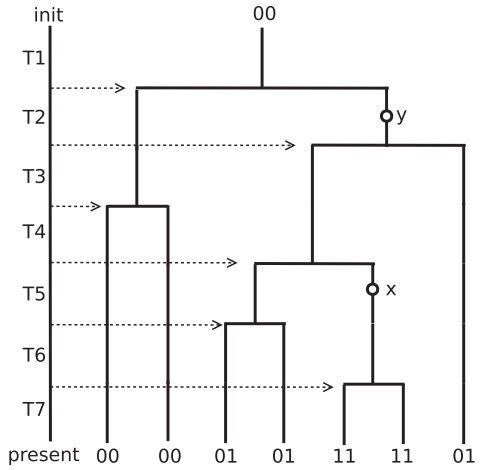
\includegraphics[width=8cm]{chaps/rw/intro_phylo}}
	\caption{نمایی از یک درخت فیلوژنیک تومور}
	\label{fig:ch_rw:intro_phylo}
\end{figure}
برای استنباط درخت فیلوژنی تومور، الگوریتم کیم و سایمون از سه بخش اصلی تشکیل شده است. طبق قضیه بیز برای محاسبه هر یک از این سه احتمال به مقادیر \gls{likelihood}  نیاز داریم. مقدار احتمال رخداد طبق رابطه‌ زیر محاسبه می‌گردد:
\begin{equation}
	P(x\sim y | D) \propto L(x\sim y)P(x\sim y), \quad L(x\sim y) = P(D|x\sim y)
\end{equation}
طبق این رابطه و با توجه به اینکه رابطه‌ زمانی میان جهش‌های \lr{x} و \lr{y} دارای 3 حالت،
\begin{equation*}
	x \rightarrow y, \qquad y \rightarrow x \qquad \text{و} \qquad x \not\leftrightarrow y
\end{equation*}
است، مقدار احتمال محاسبه شده از رابطه فوق به ازای یکی از این سه حالت بیشینه است و به ازای آن حالت یک مسیر جهت‌دار در درخت فیلوژنی قرار خواهد گرفت. طبق آنچه گفته شد یک گراف جهت دار فیلوژنی بلقوه مشابه آنچه در شکل \ref{fig:ch_rw:digraph} نشان داده ‌شده است استنباط خواهد شد. در نهایت از این گراف جهت دار، یک درخت به طوری که روابط میان جهش‌ها از آن استنباط شود ساخته خواهد شد. 
\begin{figure}[!ht]
	\centerline{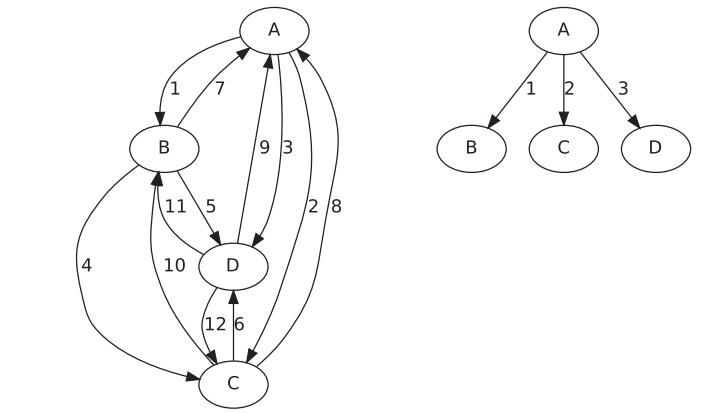
\includegraphics[width=12cm]{chaps/rw/digraph}}
	\caption{یک گراف جهت دار فیلوژنی}
	\label{fig:ch_rw:digraph}
\end{figure}
در ابتدا یال‌های گراف از طریق رابطه‌ای که در ادامه آمده است وزن‌دهی می‌شوند،
\begin{equation}
	w_{x\sim y} = -\log P(x\sim y| D)
\end{equation}
که در آن \lr{$(x \sim y)$ } رابطه بین جهش‌های $x$ و $y$ است و $D$ نمونه یا سمپل‌های موجود در داده است. بهترین درخت $\hat{T}$ از طریق کمینه‌کردن وزن‌های گراف بدست می‌آید.
\begin{equation}
	\hat{T} = \arg \min\Big( \sum_{x\sim y \in T} w_{x\sim y} \Big)= \arg \max \Big( \prod_{x\sim y \in T} P(x\sim y | D) \Big )
\end{equation}
در شکل \ref{fig:ch_rw:digraph} محتمل‌ترین \gls{phylogenytree} با بیشینه \gls{likelihood} بر اساس اطلاعات نمونه‌برداری شده بدست می‌آید. در این شکل گراف اولیه و درخت متناظر آن مشاهده می‌شود. مجموع همه وزن‌ها در درخت نهایی با شرط کمینه سازی برابر هفت است که این مقدار کمترین مقدار ممکن است. 
\subsection{پایگاه داده}
در این مقاله از پایگاه داده تولی‌یابی تک سلولی هو‌ و همکاران \cite{hou2012single} استفاده شده است. این مجموع داده از توالی‌یابی تک‌سلولی \gls{dna} نمونه‌های توموری یک نوع خاص از \gls{thrombocythemia} جمع‌آوری شده است. این مجموعه داده شامل 58 سلول منفرد و 18 نوع جهش یکتا است. اطلاعات کامل در مورد این پایگاه داده از جمله، نام و نوع جهش‌های موجود در دیتابیس، نوع روش نمونه‌برداری و اطلاعاتی دیگر در پایگاه داده \lr{COSMIC} در دسرس عموم قرار دارد. ماتریس ژنوتایپی این پایگاه داده شامل سه مقدار صفر، یک و دو می‌باشد که در آن صفر بیانگر عدم وجود جهش، یک بیانگر جهش هتروزیگوت و دو نمایانگر جهش هموزیگوت است. یکی از معایب این پایگاه داده نرخ بالای خطای توالی‌یابی تک‌سلولی و بالا‌ بودن نرخ داده‌های از دست رفته (در حدود 45 درصد کل داده‌ها) می‌باشد. همین امر سبب می‌شود تنوع \gls{phylogenytree} نسبت داده شده به این پایگاه داده زیاد باشد. در واقع با در نظر گرفتن حالت‌های مختلف روابط دو‌به‌دوی جهش‌های گوناگون، می‌توان درخت‌های جهشی متنوعی از داده‌ها استنباط کرد. 

\subsection{معیار ارزیابی}
ارزیابی درختهای جهشی گوناگون از طریق روش \lr{\gls{leaveoneoutcrossvalidation}} صورت میگیرد. این روش همانند روش ا\gls{crossvalidation} با $K$ قسمت می‌باشد با این تفاوت که در آن $k$ برابر تعداد جهش‌ها (تعداد ستون‌های ماتریس ژنوتایپ) می‌باشد. در هر یک از درخت‌های استنباط شده، یکبار یک جهش حذف شده و میزان دقت مدل محاسبه می‌گردد. سپس این کار برای همه جهش‌های موجود تکرار می‌شود و در نهایت میانگین دقت مدل در حالتهای مختلف محاسبه می‌شود و به عنوان دقت نهایی مدل گزارش می‌شود.  

\section{الگوریتم \lr{Bitphylogeny} \cite{yuan2015bitphylogeny}}
این الگوریتم در سال 2015 ارئه شد و مانند الگوریتم کیم و سایمون از منطق بیزی بهره می‌برد. هدف این الگوریتم در کنار ساخت درخت جهشی تومور، پیدا کردن روابط بین کلون‌های مختلف درون یک تومور است. در داده‌های توالی‌یابی تک‌سلولی، بدلیل کمبود میزان نمونه‌گیری و در نتیجه محتمل بودن عدم حضور گونه‌های ژنومی جهش‌یافته در نمونه‌ها، برای تشخیص ناهمگنی‌های درون توموری باید رویکرد متفاوتی را برگزید. شاید یکی از دلایلی که هنوز از داده‌های \gls{bulksequencing} برای استنباط \gls{phylogenytree} استفاده می‌شود همین باشد. در هر صورت در این مقاله سعی بر این است تا هر 2 چالش زیر مورد بررسی قرار گیرد: 
\begin{itemize}
	\item  تشخیص زیرنواحی یا کلون‌های درون یک تومور 
	\item	کشف روابط تکاملی کلونهای درون یک تومور با یکدیگر 
\end{itemize}

ماتریس ورودی (ماتریس ژنوتایپی) این الگوریتم تعدادی سطر و ستون است که در آن سطرها بیانگر سلولها و ستونها نمایانگر انواع جهشهای مختلف است. این ماتریس، یک ماتریس \gls{binary} است که در آن بودن درایه $i$ و $j$ بیانگر آن است که در سطر $i$ام جهشی از نوع $j$ ام وجود ندارد. متعاقباً، اگر مقدار درایه $i$ و $j$ برابر یک باشد در سطر $i$ام جهشی از نوع $j$ام وجود دارد. 

دراین مقاله برای جستجو درختی که بیشترین تطابق با داده‌های ورودی را داشته باشد از الگوریتم \gls{markovchainmontecarlo} استفاده می‌شود. این الگوریتم سلول‌ها با ژنوتایپ مشابه را درون یک گروه قرار می‌دهد و به این گروه‌ها کلون گفته می‌شود. در طی دسته‌بندی سلول‌ها کلون‌هایی ایجاد می‌شود که با احتمال زیاد توموری بوده ولی در نمونه‌گیری از بافت توموری حضور نداشته‌اند. شناسایی این گونه از کلون‌ها با توجه به روند گسترش و تکامل تومور، که به مرور زمان صورت می‌گیرد، امکان پذیر است. این الگوریتم قادر است تا یک تخمین زمانی از انتقال جهش از سطوح بالای \gls{phylogenytree} به سطوح پایین‌تر را محاسبه کند. در این الگوریتم از داده‌های تغییرات تک \gls{nucleotid} استفاده شده‌است اما این روش این قابلیت را دارد تا بدون در نظر گفتن فرض مکان‌های بینهایت برای داده‌های متیلاسیون \gls{dna} استفاده شود. از نکات قوت این الگوریتم می‌توان  به محاسبه رخداد هر جهش در \gls{phylogenytree} تومور اشاره کرد اما این مقدار احتمال بدلیل تعداد بالای داده‌های از دست رفته و نرخ بالای خطای \gls{falsepositive} و \gls{falsenegative}، بیش از مقدار واقعی است. 

شایان ذکر است که این الگوریتم محدودیت‌های خاص خود را دارد. به عنوان مثال، در نظر گرفتن فرض مکان‌های بینهایت برای رخداد جهش‌ها و زمان محاسباتی بسیار بالا الگوریتم \gls{markovchainmontecarlo} برای استنباط \gls{phylogenytree} از جمله این محدودیت‌ها می‌باشد. از دیگر محدودیت‌های این الگوریتم می‌توان به عدم تشخیص کلون‌های هموژنی و هتروژنی در یک نوع جهش از یکدیگر اشاره کرد. منظور از کلون‌های هموژنی در یک جهش معین آن است که اجزای تشکیل دهنده آن با توزیع یکنواخت در کنار یکدیگر قرار گرفته‌اند و این بدان معناست که احتمال رخداد هر جهش در این توده برابر با احتمال رخداد دیگر جهش‌هاست. در مقابل، یک توده دارای خاصیت هتروژنی است اگر اجزای تشکیل دهنده آن توزیع غیریکنواخت داشته باشد و به همین امر سبب می‌شود تا بدلیل حضور سلول‌های مختلف با توزیع گوناگون، احتمال رخداد جهش‌های مختلف متفاوت باشد. 

\subsection{پایگاه داده}
به منظور ارزیابی مدل استنباط کننده درخت تکاملی تومور، از دو پایگاه داده متفاوت در این مقاله استفاده شده‌است: 
\begin{itemize}
	\item دادگان مربوط به الگوهای متیلاسیون سرطان روده بزرگ
	\item دادگان شبیه‌سازی شده مربوط به سرطان خون
\end{itemize}
 

\subsection{معیار ارزیابی}
 به منظور ارزیابی عمکرد الگوریتم بیت‌فیلوژنی یک مقایسه بین خروجی این الگوریتم و خروجی‌های الگوریتم‌های \gls{kcentroids} و \gls{hierarchicalClustering} صورت گرفته است. این مقایسه از طریق محاسبه معیار بیشینه عمق درخت تکاملی استنباط شده و مقدار \gls{likelihood} صورت گرفته است. نتایج گزارش شده در این مقاله گواه از \gls{consistency} و \gls{accuracy} بسیار بهتر الگریتم بیت‌فیلوژنی  نسبت به دو الگوریتم دیگر است. در شکل \ref{fig:ch_rw:comp_1} میزان خطای عملکرد الگوریتم بیت‌فیلوژنی نسبت به دو الگوریتم \gls{kcentroids} و \gls{hierarchicalClustering} در سطوح مختلف درخت در حالت‌های تک‌کلونی و چندکلونی قابل مشاهده است.
 
\begin{figure}[!ht]
	\centerline{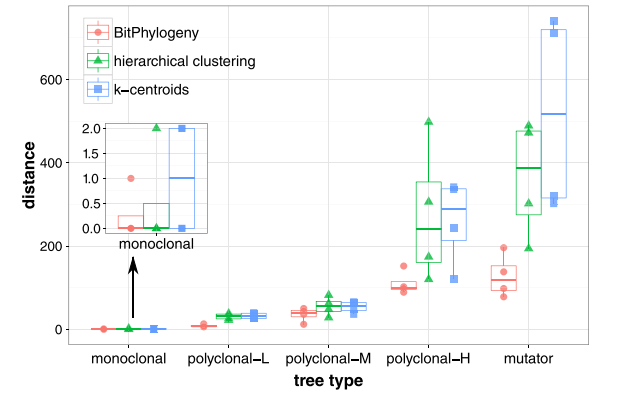
\includegraphics[width=13cm]{chaps/rw/comp_1}}
	\caption{میزان خطای عملکرد الگوریتم بیت‌فیلوژنی نسبت به دو الگوریتم \gls{kcentroids} و \gls{hierarchicalClustering} در سطوح مختلف درخت در حالت‌های تک‌کلونی و چندکلونی \cite{yuan2015bitphylogeny}}
	\label{fig:ch_rw:comp_1}
\end{figure}

در شکل \ref{fig:ch_rw:bitphylo} به طور کلی مراحل عمکلرد الگوریتم بیت‌فیلوژنی را مشاهده می‌کنید. این شکل تومور چندکلونی \lr{A} را نشان  می‌دهد که به روش توالی‌یابی نمونه‌گیری شده است. این تومور شامل سه کلون مجزا و سلول‌های سالم (دایره‌های  خاکستری رنگ) است. در تصویر میانی یک درخت بلقوه که نشان‌دهنده سیر تکاملی تومور است نشان داده شده است. در تصویر سمت راست درخت کلونی بدست آمده از درخت تکاملی تومور گفته شده با الگوریتم بیت‌فیلوژنی مشاهده می‌شود که در آن کلون‌ها و فراوانی هر یک مشهود است. 

\begin{figure}[!ht]
	\centerline{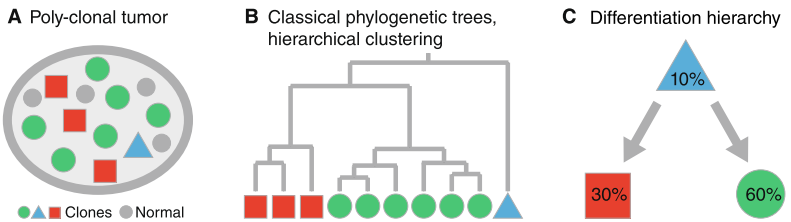
\includegraphics[width=13cm]{chaps/rw/bitphylo}}
	\caption{مراحل عمکلرد الگوریتم بیت‌فیلوژنی}
	\label{fig:ch_rw:bitphylo}
\end{figure}


\section{الگوریتم \lr{SCITE} \cite{jahn2016tree}}

این الگوریتم با استفاده از داده‌های \gls{scs} سعی در استنباط \gls{phylogenytree} تومور دارد. همانطور که پیشتر نیز اشاره شد، یک تومور ناشی از تجمع تعدادی سلول با ویژگی‌های ژنی متفاوت است و این سلول‌ها سعی دارند تا این ویژگی‌های ژنی منحصربه‌فرد را از طریق تکثیر سلولی به سلول‌های بعدی منتقل کنند.  \cite{davis2016computing}

وجود سلول‌ها با جهش‌های متفاوت سبب می‌شود که تومور از زیرنواحی گوناگون، که به کلون مشهور هستند، تشکیل شود. هر چه تومور از تعداد کمتری زیرکلون تشکیل شده باشد درمان آن ساده‌تر خواهد بود. در نظر گرفتن هر کلون به صورت یک تومور جداگانه، مطالعه و بررسی هر یک از این زیرتومورها به صورت دقیق‌تر و یافتن سیر تکاملی آنها سبب می‌شود تا درمان تومور به صورت کارآمدتری انجام شود.  \cite{beerenwinkel2015cancer}

یکی از چالش‌های بزرگ در زمینه تشخیص و مطالعه کلون‌های درون تومور، توالی‌یابی قسمت‌های مشترک دنباله‌های \gls{dna} است، زیرا شامل ترکیبهای بسیار زیادی (در حدود میلیون‌ها ترکیب) از ژنهای سلول‌های گوناگون است. جهش‌های بدست آمده از ترکیب توالی سلول‌های مختلف، با تعداد زیرنواحی توموری (کلون) متناسب است و با استفاده از تعداد زیرنواحی می‌توان تخمین نزدیکی از جهش‌های درون یک نمونه را بدست آورد \cite{mcgranahan2017clonal}. به همین دلیل به منظور شناسایی دقیق هر یک از زیرنواحی توموری (کلون‌ها) لازم است تا اطلاعات حاصل از نواحی مشترک کلون‌ها به دقت مورد تحلیل و تجزیه قرار گیرد.  \cite{salehi2017ddclone}


الگوریتم \lr{Scite} از طریق داده‌های \gls{scs} قادر است سیر تکاملی تومور را از طریق درخت جهشی تومور که درآن ترتیب وقوع جهش‌ها مشخص است یا از طریق استنباط درخت فیلوژنیک تومور که در آن هر برگ نشان دهنده یک سلول است، نشان دهد. خروجی مدل \lr{Scite} نتیجه ارزیابی بهتری در مقایسه با الگوریتم بیت‌فیلوژنی بر روی داده‌های واقعی داراست. الگوریتم \lr{Scite} از طریق معیار بیشینه \gls{likelihood} و احتمال رخداد هر جهش و با استفاده از ماتریس ژنوتایپ ورودی تعیین می‌کند که کدام درخت استنباط بهتری از سیر تکاملی تومور است. در حالتی که تعداد جهش‌ها بسیار زیاد باشد یعنی تعداد ستون‌های ماتریس ژنوتایپ ورودی زیاد باشد، ساخت درخت فیلوژنیک راحت‌تر خواهد بود، اما در حالتی که تعداد سلولها زیاد باشد (تعداد سطرهای ماتریس ژنوتایپپ بالا باشد) ساخت درخت جهشی تومور (ترتیب وقوع جهش‌ها) راحت‌تر است. به طور خلاصه اینکه کدام نوع درخت ( جهشی یا فیلوژنیک) در نهایت بیان‌کننده سیر تکاملی تومور باشد به نرخ جهش‌های توموری و روش توالی‌یابی داده‌ها بستگی دارد.  
\\
در الگوریتم \lr{Scite} از دو فرض اصلی استفاده می‌شود: 
\begin{itemize}
	\item     فرض \gls{infinitesites} که بر طبق آن هر جهش تنها یکبار در هر موقعیت از ژنوم رخ ‌می‌دهد. 
	\item	فرض جهش‌های نقطه‌ای یعنی مدل تکاملی تومور به جهش‌های نقطه‌ای محدود می‌شود.  
\end{itemize}
مانند الگوریتم بیت‌فیلوژنی از یک ماتریس ژنوتایپ (ماتریس \gls{binary} که سطرها نمایانگر نمونه‌ها و ستون‌ها بیانگر جهش‌هاست) به عنوان ورودی الگریتم استفاده می‌شود. موقعیت هر جهش به صورت درایه $i$ و $j$ از ماتریس $n*m$ مشخص می‌شود. به این صورت که مقدار صفر در سطر $i$ام و درایه $j$ام بیانگر آن است که جهش از نوع $j$ در سطر $i$ وجود ندارد. یک ماتریس ژنوتایپ را \gls{perfectphylogenicmatrix} گوییم هر گاه به ازای آن یک درخت فیلوژنیک متناظر باشد. در الگوریتم \lr{scite} همانند الگوریتم بیت‌فیلوژنی از الگوریتم \gls{markovchainmontecarlo} برای اسنباط درخت تتکاملی تومور از داده‌های \gls{scs} استفاده می‌شود، با این تفاوت که فضای جستجو برای انتخاب پارامترها بسیار محدودتر از حالت بیت‌فیلوژنی است و نرخ خطاهای داده (\gls{falsepositive} و \gls{falsenegative}) برای همه جهش‌ها یکسان در نظر گرفته شده است. محدود کردن فضا جستجو برای انتخاب پارامترها از طریق نمونه‌برداری در این فضا، سبب می‌شود تا بر اساس سیر زمانی جهش، بیشینه \gls{likelihood} از روی توزیع احتمال پیشین نمونه‌ها بدست آید. یکی از مزایای این روش محاسبه نرخ خطا توالی‌یابی است. شکل \ref{fig:ch_rw:scite_intro} یک استنتاج تکاملی از داده‌های \gls{scs} را نشان می‌دهد. در این شکل، \lr{a} یک \gls{perfectphylogenicmatrix} است اما \lr{g} ماتریس داده‌های واقعی است که شامل مقادیر از دست‌رفته، خطای \gls{falsepositive} و خطای \gls{falsenegative}  است. ماتریس داده‌های واقعی با $D$ و \gls{perfectphylogenicmatrix} را با $E$ نشان داده شده است.
 
\begin{figure}[!ht]
	\centerline{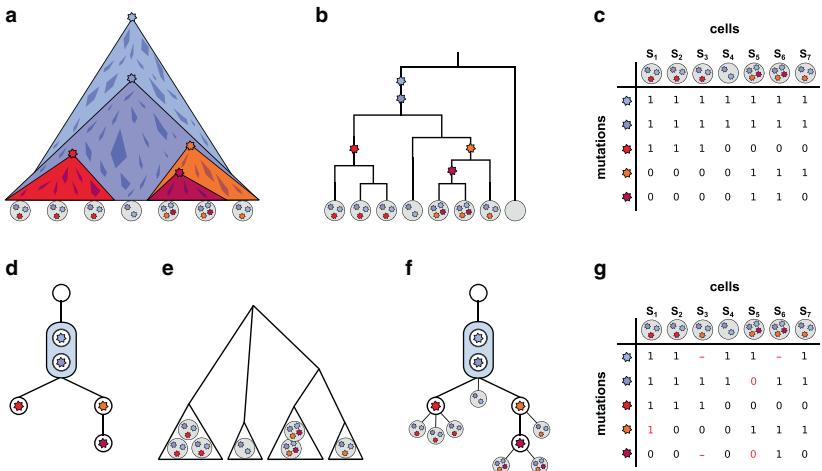
\includegraphics[width=14cm]{chaps/rw/scite_intro}}
	\caption{یک استنتاج تکاملی از داده‌های \gls{scs} \cite{jahn2016tree}}
	\label{fig:ch_rw:scite_intro}
\end{figure}

منظور از خطای \gls{falsepositive} این است که به عنوان مثال در یک موقعیت خاص از ماتریس \lr{E} جهشی وجود ندارد (مقدار ماتریس برابر صفر است) اما در همین موقعیت مقدار یک ( وجود جهش) در ماتریس \lr{D} وجود دارد. نرخ خطای \gls{falsepositive} با  $\alpha$ و نرخ خطای \gls{falsenegative} با $\beta$ نشان داده می‌شود. مقادیر $\alpha$ و $\beta$ از طریق روابط \ref{eq:ch_rw:alpha_beta} تعریف می‌گردند.
\begin{equation}
	\begin{aligned}
		&P(D_{ij}=1|E_{ij}=0)=\alpha, &\qquad P(D_{ij}=0|E_{ij}=0)=1-\alpha \\ &P(D_{ij}=0|E_{ij}=1)=\beta, &\qquad P(D_{ij}=1|E_{ij}=1)=1-\beta
	\end{aligned}
	\label{eq:ch_rw:alpha_beta}
\end{equation}

 در این معادلات فرض بر استقلال نرخ خطاهای مشاهده شده است. مقدار \gls{likelihood} درخت جهشی \lr{T} با بردار ضمیمه $\partial$ و نرخ خطای $\theta = (\alpha, \beta)$ به صورت زیر محاسبه می‌گردد. 
 \begin{equation}
 	y=xxxxxxxxxxxxxxxxxxxxxxxxxxxxxxxxxx
 \end{equation}
 
 در معادله بالا \lr{E} ماتریس جهش‌دار است که با درخت جهشی \lr{T} و بردار ضمیمه $\partial$  تعریف می‌گردد. توزیع احتمال پسین به صورت زیر محاسبه می‌گردد: 
 \begin{equation}
	y=xxxxxxxxxxxxxxxxxxxxxxxxxxxxxxxxxx
\end{equation}

به منظور بالا رفتن سرعت همگرایی مدل \gls{markovchainmontecarlo} فرض می‌شود که بردار ضمیمه $\partial$ توزیع یکنواخت دارد. در نتیجه: 

 \begin{equation}
	y=xxxxxxxxxxxxxxxxxxxxxxxxxxxxxxxxxx
\end{equation}


اندازه فضای جستجو برای دو پارامتر درخت جهشی \lr{ T} و بردار ضمیمه $\partial$ برابر با \lr{$(n+1)^{n-1}\times(n+1)^m$} می‌باشد. این فضا جستجو با فرض یکنواخت بودن توزیع بردار ضمیمه $\partial$ و طبق معادله بالا و حذف بردار ضمیمه به \lr{$(n+1)^{n-1}$} انتخاب کاهش می‌یابد. پس از همگرایی با استفاده از الگوریتم \gls{markovchainmontecarlo} و احتمال پسین، بهترین ترکیب درخت جهشی \lr{T} با بردار ضمیمه $\partial$ با بیشینه \gls{likelihood} بدست می‌آید: 
 \begin{equation}
	y=xxxxxxxxxxxxxxxxxxxxxxxxxxxxxxxxxx
\end{equation}

منظور از \lr{MAP} در این معادله حالتی است که بیشینه \gls{likelihood} رخ داده است.  

\subsection{پایگاه داده}

به منظور ارزیابی عملکرد الگوریتم \lr{Scite} برای استنباط درخت تکاملی تومور از داده‌های \gls{scs} از داده‌های واقعی و شبیه‌سازی شده، استفاده شده است. مجموعه داده‌های استفاده شده جهت ارزیابی الگوریتم عبارتند از: 

\begin{itemize}
	\item      داده‌های  \gls{scs} از یک نمونه تومور مغز استخوان با 58 سلول سرطانی و 18 نوع جهش با نرخ خطای مثبت کاذب $6.4\times10^{-4}$ و نرخ خطا    منفی کاذب $ 0.4309$ . 
	\item     داده‌های  \gls{scs} یک نوع خاص از سرطان کبد با 17 سلول سرطانی و 50 نوع جهش با مقادیر نرخ خطای مثبت کاذب  $2.67 \times 10^{-5}$ و نرخ خطا منفی کاذب $0.1643$ و نرخ داده‌های از دست رفته 22 درصد. 
	\item     داده‌های \gls{scs}نمونه‌گیری شده از سرطان سینه با 47 سلول سرطانی و 40 نوع جهش و با نرخ خطای \gls{alleledropout} 73 درصد و نرخ خطای مثبت کاذب $1.24 \times 10^{-6}$ . 
\end{itemize}


شایان ذکر است که مدت زمان استنباط یک \gls{phylogenytree} تا حد زیادی به پیچیدگی داده‌های ورودی بستگی دارد بطوریکه برای ساخت یک درخت با 50 تا 100 سلول، مدت زمانی در حدود چندین دقیقه طول می‌کشد. از مهمترین محدودیت‌های این الگوریتم می‌توان به فرض \gls{infinitesites} اشاره کرد، زیرا این امکان وجود دارد که در یک محل مشخص از یک دنباله \gls{dna}، یک جهش مشخص چندین بار رخ دهد و یا در محل‌های مختلف از یک دنباله ژنی جهش‌های مشابه رخ دهد که این موارد در فرض \gls{infinitesites} در نظر گرفته نمی‌شود. از دیگر محدودیت‌های این روش آن است که جهش‌هایی که در همه سلول‌ها وجود دارند یا جهش‌هایی که فقط در یک سلول مشاهده شده‌اند (سطری با مقادیر تماماً یک در ماتریس ورودی) در روند استنباط درخت مورد استفاده قرار نمی‌گیرند. 


\section{الگوریتم \lr{Onconem} \cite{ross2016onconem}}

%توده‌های سرطانی حاصل تجمیع کلون‌های متفاوت هستند که کلون‌ها متشکل از سلول‌هایی با جهش‌های ژنتیکی مشابه می‌باشند. وجود زیرنواحی با جهش‌های ژنتیکی متفاوت و جمعیت‌های سلولی گوناگون منجر به مقاوم شدن تومور در برابر درمان‌های دارویی شده و روند درمان تومور را دچار اختلال می‌کند زیرا که هر یک از داروها به طور موثر یک زیرناحیه توموری را هدف قرار می‌دهد. عدم درمان کامل زیرنواحی توموری می‌تواند منجر به عود مجدد تومور شود. به همین منظور نیاز به یک متد درمان بهینه به گونه‌ای که همه ناحیه‌های کلونی تومور را به طور موثر تحت تاثیر قرار دهد، بیش از پیش احساس می‌شود.  \cite{ross2016onconem}

این الگوریتم در سال 2016 با هدف یافتن تاریخچه تکاملی ناحیه‌های درون توموری با استفاده از داده‌های \gls{scs} ارائه گردید. این الگوریتم قادر است تا ناحیه‌های درون توموری مشابه را درون یک دسته قرار دهد و برای آنها یک ژنوتایپ یکتا در نظر بگیرد. این الگوریتم بر مبنای تغییرات تک نوکلئوتیدی، درخت تکاملی تومور را استنباط می‌کند و قادر به یافتن خطاهای ژنوتایپی می‌باشد. در نهایت با ارزیابی بر روی داده‌های آزمایش، مدل نهایی سنجیده شده و سلول‌ها با جهش‌های یکسان در یک گروه دسته‌بندی شده و در انتها رابطه میان جهش‌ها و ژنوتایپ‌های مشاهده شده و مشاهده نشده (پیش‌بینی شده) مشخص می‌گردد. این الگوریتم هم می‌تواند درخت کلونال توموری و هم درخت فیلوژنیک توموری ( قرارگرفتن سلول‌ها به عنوان برگهای درخت) را به عنوان خروجی بدست دهد. ورودی این الگوریتم ماتریس دودویی ژنوتایپ به همراه نرخ خطا مثبت کاذب و نرخ خطا منفی کاذب و نرخ خطا داده‌های از دست رفته است. در ادامه، الگوریتم سعی می‌کند تا سلول‌ها با ژنوتایپ‌های مشابه را در یک گروه قرار دهد و در نهایت درختی که بیشترین شباهت را با دسته‌بندی صورت گرفته را دارد به عنوان درخت تکاملی تومور استنباط کند. از نکات قوت این الگوریتم آن است که قادر است کلون‌هایی را که احتمال وجود آنها بالاست اما در داده‌های نمونه‌گیری شده حضور ندارند حدس بزند. این الگوریتم از دو قسمت اصلی تشکیل شده است: 
\begin{itemize}
	\item ایجاد یک مدل احتمالاتی به منظور مدل کردن جمیع جهش‌ها بر مبنای داده‌های نویزی و روابط میان داده‌ها 
	\item پیدا کردن درخت‌هایی با بیشترین میزان \gls{likelihood} در فضای جستجو 
\end{itemize}
توزیع احتمال پسین با فرض \lr{D} به عنوان مجموعه داده‌های مدل به صورت زیر محاسبه می‌گردد
\begin{equation}
	y=xxxxxxxxxxxxxxxxxxxxxxxx
\end{equation}

که در آن $\tau$ نمایانگر یک درخت جهش‌دار (که نباید حتماً دودویی باشد) است که ریشه آن یک گره سالم و بدون جهش است و $\theta$ یک بردار رخداد است. در این رابطه فرض بر آن است که $p(\tau)$ دارای توزیع یکنواخت است. رابطه بالا می‌تواند به شکل زیر بازنویسی شود

\begin{equation}
	y=xxxxxxxxxxxxxxxxxxxxxxxx
\end{equation}

بر طبق این رابطه، برای درختی با  $n$ راس، فضا جستجو شامل $n^{n-2}$  انتخاب است که هزینه محاسباتی بسیار بالایی برای درختانی با راس‌های بیشتر از 9 دارد. طبق شکل \ref{fig:ch_rw:onconem}، برای محدود کردن فضای جستجو از یک الگوریتم اکتشافی استفاده می‌شود تا اطمینان حاصل شود که خروجی الگوریتم یک نقطه بهینه محلی نباشد. نقطه قوت این الگوریتم سرعت بالای استنباط درخت برای داده‌های کم است ولی در مقابل از محدودیت‌های آن می‌توان به فرض بینهایت اشاره کرد.

\begin{figure}[!ht]
	\centerline{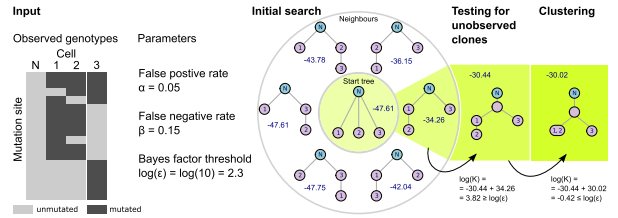
\includegraphics[width=14cm]{chaps/rw/onconem}}
	\caption{نمای شماتیکی از الگوریتم \lr{Onconem} \cite{ross2016onconem}}
	\label{fig:ch_rw:onconem}
\end{figure}

روند کلی الگوریتم \lr{Onconem} در شکل بالا توضیح داده است. طبق این شکل، ماتریس دودویی ژنوتایپی به همراه نرخ خطاهای $\alpha$ و $\beta$ به عنوان ورودی الگوریتم استفاده می‌شوند. طبق شکل بالا میزان \gls{likelihood} اولیه برابر $-47.61$  محاسبه شده است اما از میان همه درخت‌های همسایه درخت اولیه، آن درختی که بیشترین \gls{likelihood} را دارد به عنوان درخت اولیه انتخاب می‌شود (با \gls{likelihood} $-36.26$). در ادامه یک گرهای که احتمال رخداد آن طبق ماتریس ورودی بالاست ولی در داده‌های ورودی وجود ندارد به درخت اضافه می‌شود. در این حالت مقدار \gls{likelihood} به $3.82$ افزایش می‌یابد و این کلون مشاهده نشده بدلیل بزرگتر بودن مقدار \gls{likelihood} از آستانه تعیین شده، به مدل افزوده می‌شود. در نهایت گره‌های یک شاخه تا جایی که سبب کاهش میزان \gls{likelihood} نشوند، در یک کلون تجمیع می‌شوند. 
\subsection{پایگاه داده}

به منظور ارزیابی عملکرد الگوریتم \lr{Onconem} از دو پایگاه داده مجزا استفاده شده است
\begin{itemize}
	\item     داده‌های  \gls{scs} مربوط به سرطان مثانه که شامل 44 سلول سرطانی است. در حدود 55 درصد از انواع جهش‌های موجود در این پایگاه داده، اطلاعاتی در دسترس نیست یعنی بیش از نیمی از داده‌های موجود از \gls{missingdata}‌اند . خروجی الگوریتم \lr{Onconem} برای این پایگاه داده یک درخت فیلوژنی با سه کلون اصلی می‌باشد و یک چهارم سلول‌های جهش‌یافته را شامل می‌شود.  
	\item     داده‌های مربوط به سرطان خون که در مدل کیم و سایمون و الگوریتم بیت‌فیلوژنی از آن استفاده شده بود، در این ارزیابی مورد استفاده قرار گرفت. میزان لگاریتم \gls{likelihood} الگوریتم \lr{Onconem} برای این مجموع داده برابر $-9964$ گزارش شده است که بالاتر از مقداری است که الگوریتم بیت‌فیلوژنی به آن رسیده بود ($-11584$).  
\end{itemize}


\section{الگوریتم \lr{Sasc} \cite{ross2016onconem}}
سرطان ناشی از جهش‌های ژنومیک یک سلول است که این جهش‌ها به مرور زمان رشد و تکثیر می‌یابند و زیرنواحی متفاوتی را ایجاد می‌کنند. این زیرنواحی، که به آنها کلون نیز گفته می‌شود، خصویات متفاوتی دارند و در کنار هم یک توده سرطانی را تشکیل می‌دهند. بررسی تاریخچه تکاملی تومور می‌تواند کارآمدی درمان‌های موجود را بهبود بخشد و امکان عود مجدد تومور را تا حد زیادی کاهش دهد. به منظور درک بهتر تاریخچه تکاملی تومور فرض‌های گوناگونی جهت ساده‌سازی مسئله صورت می‌گیرد، مثل فرض \gls{infinitesites} که طبق آن هر جهش یکتایی تنها یکبار رخ می‌دهد. مطالعات زیادی صورت گرفته است که نشان می‌دهد در نظر گرفتن فرض \gls{infinitesites} به تنهایی برای استنباط روند تکاملی تومور کافی نیست و محدودیت‌هایی دارد، به همین منظور برای درک بهتر نواحی ناهمگن توموری باید فرض‌های دیگری را به مسئله اضافه کنیم. به همین دلیل یک فرضیه جدید تحت عنوان \lr{k-dollo} ارائه گردید که بر طبق آن و بر خلاف فرض \gls{infinitesites}، هر جهشی تنها یکبار رخ می‌دهد اما امکان از دست دادن این جهش به تعداد \lr{k} در تاریخچه تکاملی تومور وجود دارد. الگوریتم \LR{Sasc} که در سال 2018 ارائه گردید، از اولین الگوریتم‌هایی بود که از فرض \lr{k-dollo} جهت استنباط درخت تکاملی تومور بهره برد. به مانند الگوریتم \lr{Onconem}، این الگوریتم به منظور محدود کردن فضای جستجو از یک الگوریتم درخت اکتشافی بهره می‌برد. الگوریتم اکتشافی استفاده شده در این روش، الگوریتم شبیه‌سازی ذوب فلزات است و هدف آن پیدا کردن بیشینه \gls{likelihood} برای تابع احتمال رخداد پسین در فضا جستجو است. طبق این الگوریتم، ابتدا از طریق مجموعه‌ای از انتخاب‌های نمونه‌برداری شده از فضا جستجو یک راه‌حل برای مسئله ارائه می‌گردد. اگر مقدار \gls{likelihood} نسبت به حالت اولیه بهبود یافته بود، با احتمال یک پذیرفته می‌شود در غیر این صورت احتمال رخداد آن حالت صفر در نظر گرفته می‌شود. این الگوریتم سعی دارد تا بیشینه \gls{likelihood} ماتریس ژنوتایپ ورودی را حساب کند. ورودی این الگوریتم در کنار ماتریس ژنوتایپ، نرخ خطای مثبت کاذب، نرخ  خطای منفی کاذب و نرخ خطای \gls{missingdata} است و بیشینه \gls{likelihood} از رابطه زیر بدست می‌آید: 

\begin{equation}
	y=xxxxxxxxxxxxxxxxxxxxxxxxxxx
\end{equation}

\subsection{پایگاه داده: }

به منظور ارزیابی عملکرد الگوریتم \lr{Sasc} از دو پایگاه داده مجزا استفاده شده است: 
\begin{itemize}
	\item داده‌های \gls{scs} سرطان مثانه
    \item داده‌های شبیه‌سازی شده \gls{thrombocythemia} 
\end{itemize}
خروجی الگوریتم در مقایسه با الگوریتم \lr{Scite} از مقدار بیشینه \gls{likelihood} بیشتری برای مدل کردن داده‌ها برخوردار است. 


\section{الگوریتم \lr{Scarlet} \cite{satas2020scarlet}}

%سرطان فرایند تکاملی است که سلول‌های داخل یک تومور به مرور زمان جهش های \gls{somatic} تجمیع‌شونده خواهند داشت. اگرچه تنها تعداد کمی از این جهش‌های \gls{somatic} منجر به توسعه سرطان می‌شوند، با این حال تمام جهش‌های \gls{somatic} می‌توانند به عنوان یک \gls{biomarker} برای \gls{inference} تاریخچه تکامل سرطان استفاده شوند. تکنولوژی‌های اخیر \gls{scs} \gls{dna}، قابلیت اندازه‌گیری جهش‌های \gls{somatic} را در سلول‌های منفرد یک تومور ممکن می‌سازند
%
%از انجایی که ابزارهای اندازه‌گیری \gls{scs} \gls{dna}، اندازه‌گیری \gls{snvv}  را با نرخ بالای \gls{falsepositive} و \gls{falsenegative} انجام می‌دهند و همچنین \gls{snvv} تنها نوع جهش \gls{somatic} در سرطان نیستند، جهش‌های \gls{cna}  که کارشان کپی کردن یا حذف قسمت‌هایی از ژنوم است، نیز قابل شناسایی هستند. 
%
%\gls{snvv} و جهش‌های \gls{cnv}، نشانگرهای زیستی تکامل سرطان هستند. هر دو جهش \gls{snvv} و تغییر تعداد کپی در طول تکامل سرطان تجمیع خواهند شد و این جهش‌ها ممکن است در ژنوم همپوشانی داشته باشند. به عنوان مثال حذف یا پایان یک جهش ممکن است منجر به حذف \gls{snvv}‌ها نیز شود. از انجایی‌ که مدل \gls{infinitesites} اجازه حذف \gls{snvv} را نمی‌دهد، روش‌هایی که از این مدل استفاده می‌کنند به صورت دقیق \gls{phylogenytree} را با حضور \gls{cnv}ها بازسازی نخواهند کرد. 

مدل ارائه شده در این مقاله که در سال 2020 به چاپ رسیده است، یک مدل تکاملی است که امکان حذف هر نوع جهشی را  \gls{losssupported} در نظر می‌گیرد.  این مدل اجازه حذف \gls{snvv} را تنها هنگامی که با شواهد داده \gls{scs} \gls{dna} از یک حذف در همان \gls{loci} همراه شده باشد، می‌دهد. این مدل پایه الگوریتم اسکارلت خواهد بود که فیلوژنی تومور را از داده توالی یابی تک سلولی \gls{dna} با احتساب هر دوی خطای توالی‌یابی و حذف جهش‌ها نتیجه می‌دهد. 
تعداد کمی از جهش‌های سوماتیک منجر به پیشروی سرطان می‌شوند، اما تمام جهش‌های سوماتیک نشانگرهای زیستی تاریخچه تکامل تومور هستند. روشهای غالب ساخت فیلوژنی داده \gls{scs} \gls{dna} از \gls{snvv}ها به عنوان نشانگرهای زیستی استفاده می‌کنند اما در به حساب آوردن تغییر تعداد کپی، که ممکن است با \gls{snvv} همپوشانی داشته باشد و منجر به حذف \gls{snvv} شود، ناتوان است. 
الگوریتم پیشنهادی اسکارلت، فیلوژنی تومور را از داده \gls{scs} \gls{dna}، خطای توالی‌یابی و حذف \gls{snvv} از طریق تغییر تعداد کپی را لحاظ می‌کند.این الگوریتم عملکرد بهتری نسبت به روشهای موجود بر روی داده‌های شبیه‌سازی شده دارد. \gls{scs} \gls{dna} از تومور بدلیل افزایش بازدهی الگوریتم و کاهش هزینه ایزوله کردن، نشانه‌گذاری و توالی‌یابی سلول‌های انفرادی از محبوبیت روزافزونی برخوردار است. 
%
%این روش از پیچیدگی بازسازی فیلوژنی با نمونه‌گیری‌های فراوان از سلول‌ها را جلوگیری می‌کند. شایان توجه است که نمونه‌برداری تک‌سلولی به علت خطای توالی‌یابی، نمونه‌برداری کمتر و خطای تشدید \gls{dna}، خطای \gls{missingdata} را بالاتر خواهد برد. \\
%یکی از چالش‌های ساخت فیلوژنی با استفاده از داده‌های \gls{scs} \gls{dna}، که از \glspl{snvv} به عنوان نشانگر زیستی استفاده می‌کند، نرخ بالای خطای  \gls{alleledropout} (تا 30 درصد) هست. به همین منظور باید بتوان مدل تکاملی فیلوژنی را همزمان با در نظر گرفتن داده‌های ورودی از بین‌رفته ساخت. شکل \ref{fig:ch_rw:scarlet_D} نمونه ماتریس داده‌ها را نشان می‌دهد. عدد صفر به معنای عدم وجود جهش و عدد یک به معنای جهش برای سلول مورد نظر است.
%
%\begin{figure}[!ht]
%	\centerline{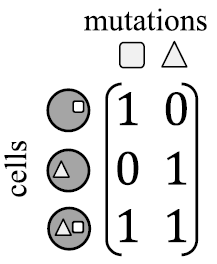
\includegraphics[width=3cm]{chaps/rw/scarlet_D}}
%	\caption{عنوانننننننننننننننننننننننننننننننننن}
%	\label{fig:ch_rw:scarlet_D}
%\end{figure}
%
%
%اگر داده‌های توالی‌یابی عاری از هر گونه خطا باشند، \gls{perfectphylogeny} بدست خواهد آمد. با در نظرگرفتن وجود خطا در ماتریس فیلوژنی و کاهش خطاهای موجود، می‌توان مدل فیلوژنی کامل را ساخت. از آنجایی که حالت‌های متعددی از تصحیح‌های متعدد امکان‌پذیر است، امکان استنباط چندین فیلوژنی گوناگون سازگاز با داده‌ها وجود دارد. با استفاده از مدل \gls{infinitesites} و اصلاح خطاها می‌توان درخت‌های فیلوژنی‌های کامل \ref{fig:ch_rw:scarlet_multians} را ساخت. در اینجا 6 درخت ممکن است.
%
%
%\begin{figure}[!ht]
%	\centerline{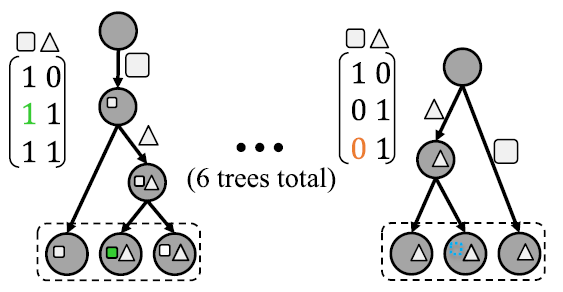
\includegraphics[width=8cm]{chaps/rw/scarlet_multians}}
%	\caption{عنوانننننننننننننننننننننننننننننننننن}
%	\label{fig:ch_rw:scarlet_multians}
%\end{figure}

شکل \ref{fig:ch_rw:scarlet_dolo} فیلوژنی با فرض \gls{dollo} را نشان می‌دهد. این مدل با شناسایی حذف جهش‌ها به منظور رفع تناقض مدل  \gls{infinitesites} می‌تواند درخت‌های \ref{fig:ch_rw:scarlet_dolo} را بسازد. هر دو مدل دولو و \gls{infinitesites} می‌توانند چندین درخت ممکن را بسازند. 
\begin{figure}[!ht]
	\centerline{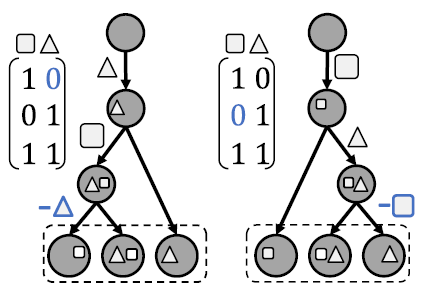
\includegraphics[width=7cm]{chaps/rw/scarlet_dolo}}
	\caption{عنوانننننننننننننننننننننننننننننننننن}
	\label{fig:ch_rw:scarlet_dolo}
\end{figure}
حتی در حالت های ساده ای که خطا وجود ندارد، استنباط چندین فیلوژنی سازگار با داده‌ها ممکن است وجود داشته باشند. در صورتی که خطا وجود داشته باشد و عدم قطعیت در ماتریس جهش وجود داشته باشد، تعداد این درخت‌های احتمالی بسیار بیشتر خواهد شد. خطای داده \gls{scs} \gls{dna} و حذف جهش‌ها منجر به پیچیدگی مسئله و ابهام در استنباط فیلوژنی خواهد شد. به عنوان مثال با مشاهده کردن 0 در ماتریس جهش به جای 1 نمی‌توان براحتی بین خطاهای داده‌ها و حذف جهش‌ها تفاوتی قائل شد. عمده محدودیت الگوریتم‌های دولو یا \gls{infinitesites}ایی که اجازه حذف جهش‌ها را می‌دهند این است که هیچکدام از این روش‌ها شواهد تغییر تعداد کپی در حذف جهش‌ها را در یک  \gls{loci} در نظر نمی‌گیرند. مدل‌های \gls{multistate} از تکامل تومور که از داده‌های توالی‌یافته با نمونه‌های زیادی از تومور استفاده می‌کنند. این نگرش‌ها نه خطای موجود در داده \gls{scs} \gls{dna} را مدل می‌کنند و نه در ابعاد صدها یا هزاران سلول قابلیت مدل کردن را دارند. 

از آنجایی که حذف جهش‌ها پیچیده‌ترین قسمت در تکامل \gls{snvv} است و مسئول اکثر تناقضات در مدل \gls{infinitesites} در داده‌های \gls{scs} \gls{dna} هستند، در نگرش ارائه شده در این الگوریتم، حذف جهش‌ها را با  استفاده از داده‌های جهش‌های تغییر تعداد کپی از همان سلول‌ها محدود خواهد کرد. در نتیجه الگوریتم اسکارلت با یکپارچه کردن \gls{snvv} و داده‌های \gls{cnv}، درخت فیلوژنی را براساس داده \gls{scs} \gls{dna}  می‌سازد. الگوریتم اسکارلت براساس مدل فیلوژنی \gls{losssupported} است که حذف جهش‌ها را محدود به مکان‌های هندسی خواهد کرد. به عنوان مثال در این الگوریتم  داده تغییر تعداد کپی گواه یک حذف است. شکل زیر مدل فیلوژنی با در نظر گرفتن خطا حذف را نشان می‌دهد که با استفاده از داده تغییر تعداد کپی  سعی در محدود کردن حذف جهش ها دارد تا بتواند \gls{conflict} ایجاد شده را رفع کند. 

\begin{figure}[!ht]
	\centerline{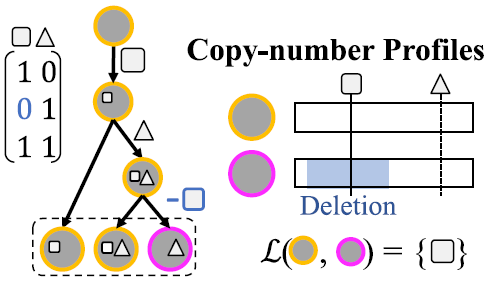
\includegraphics[width=8cm]{chaps/rw/scarlet_cnv}}
	\caption{عنوانننننننننننننننننننننننننننننننننن}
	\label{fig:ch_rw:scarlet_cnv}
\end{figure}


zzzzzzzzzzzzzzzzzzzzzzzzzzzzzzzzzzzzzzzz

مدل فیلوژنی \gls{losssupported}،  مدلی از تکامل \gls{snvv} است که جهش حداکثر یکبار رخ خواهد داد (0--à1) اما حذف جهش‌ها (0-à1) توسط مجموعه
𝓛
از مقدار خطا حذف که توسط تغییر تعداد کپی‌ها تعریف می‌شوند محدود خواهد شد. برای هر جفت سلول
𝒄,𝒄′
از مجموعه جهش‌های تغیررات تعداد کپی، مجموعه خطا به صورت
𝓛𝒄,𝒄′
تعریف خواهد شد. مدل فیلوژنی \gls{losssupported}، توسعه‌دهنده مدل‌های \gls{infinitesites} و \gls{dollo} می‌باشد. ضمنا الگوریتم اسکارلت متکی بر مدل احتمالاتی تعداد خوانش‌ها برای هر \gls{snvv} است تا خطاها و داده‌های از بین‌رفته، که در  \gls{scs} \gls{dna} معمول هستند، را مورد توجه قرار می‌دهد. 

اسکارلت سه ویژگی مهم دارد: 

\begin{itemize}
	\item     مدل فیلوژنی \gls{losssupported}، حذف جهش ها را محدود به مکان‌هایی می‌کند که کاهش متناظر با آن در تعداد جهش‌های کپی وجود داشته باشد. 
	
	\item 	این الگوریتم با استفاده از مدل فیلوژنی \gls{losssupported}، ابتدا درخت فیلوژنی اولیه استنتاج شده را پایش  و سپس از طریق داده‌های تغییر تعداد کپی، فیلوژنی نهایی را استنباط می‌کند. 
	\item	استنتاج مبتنی بر بیشینه  \gls{likelihood}  از \glspl{snvv} با استفاده از مدل احتمالاتی تعداد خوانش‌های مشاهده شده در داده‌های   \gls{scs} \gls{dna} توسط الگوریتم اسکارلت اجرا می‌شود.  
\end{itemize}




اگر تعدادی جهش‌های \gls{cnv} موجود باشند و  وضعیت جهش‌های تغییر تعداد کپی را با رنگ قرمز و حذف نواحی ژنوم در طول کل ژنوم را با رنگ آبی نشان دهیم:


\begin{figure}[!ht]
	\centerline{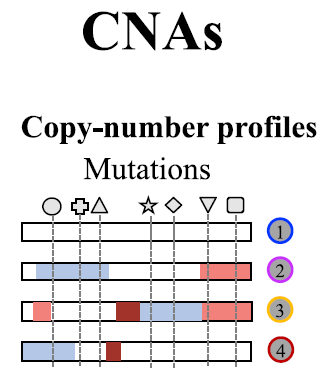
\includegraphics[width=8cm]{chaps/rw/scarlet_cna}}
	\caption{عنوانننننننننننننننننننننننننننننننننن}
	\label{fig:ch_rw:scarlet_cna}
\end{figure}

آنگاه مجموعه خطا مدل فیلوژنی \gls{losssupported}، توسط مجموعه‌های \ref{fig:ch_rw:loss_region} نمایش داده خواهد شد: 

\begin{figure}[!ht]
	\centerline{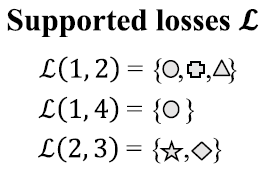
\includegraphics[width=5cm]{chaps/rw/supported_losses}}
	\caption{عنوانننننننننننننننننننننننننننننننننن}
	\label{fig:ch_rw:supported_losses}
\end{figure}

\begin{figure}[!ht]
	\centerline{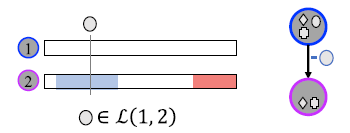
\includegraphics[width=9cm]{chaps/rw/loss_region}}
	\caption{عنوانننننننننننننننننننننننننننننننننن}
	\label{fig:ch_rw:loss_region}
\end{figure}


الگوریتم اسکارلت به صورت مستقیم وضعیت جهش‌های \gls{cnv} سلول‌های پدری را نشان نخواهد داد. به منظور غلبه بر این موضوع یک درخت برای جهش‌های \gls{cnv} زیر را در نظر خواهد گرفت که از روی وضعیت جهش‌های \gls{cnv} سلو‌‌ل‌های مشاهده شده، ساخته شده است. 


\begin{figure}[!ht]
	\centerline{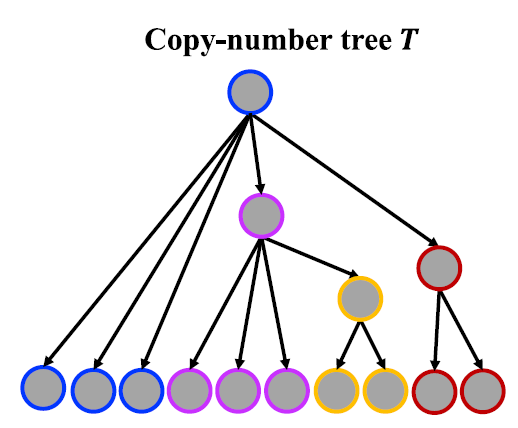
\includegraphics[width=12cm]{chaps/rw/cn_tree}}
	\caption{عنوانننننننننننننننننننننننننننننننننن}
	\label{fig:ch_rw:cn_tree}
\end{figure}


دو ورودی برای الگوریتم اسکارلت در نظر گرفته می‌شود: 
\begin{itemize}
	\item مجموعه خطاهای ناشی از حذف جهش‌ها است، که مجموعه‌های تهی در آن نمایش داده نمی‌شوند. این مجموعه جهش‌هایی که تحت تاثیر حذف قرار می‌گیرند را نشان می‌دهند. 
	\item یک درخت فیلوژنی برای جهش‌های تغییر تعداد کپی، که با استفاده از آن می‌توان روابط بین سلول‌های مشاهده شده (برگها) را آنگونه که توسط وضعیت جهش‌های تغییر تعداد کپی تعیین شده، نشان داد.
\end{itemize}


 

  

برای \glspl{snvv} \gls{variant}  \lr{X} و  \gls{total} \lr{Y}  از  \gls{readcounts} برای هر سلول و هر جهش مطابق ماتریس \ref{fig:ch_rw:scarlet_vaf} تهیه شده است: 

\begin{figure}[!ht]
	\centerline{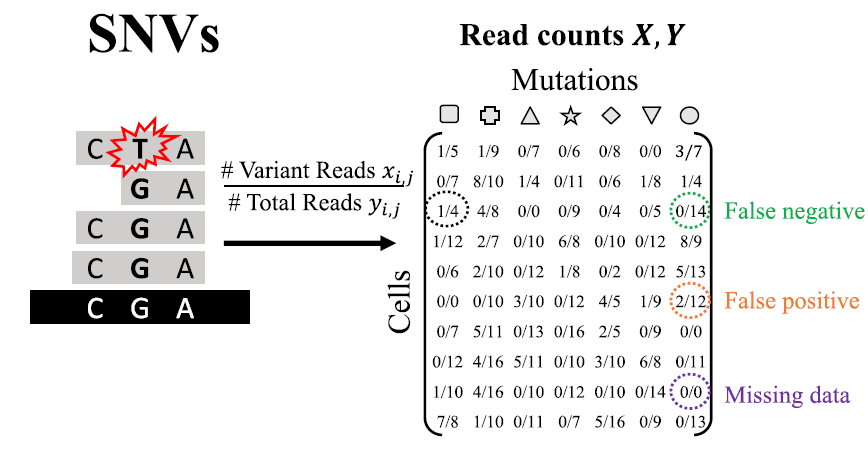
\includegraphics[width=12cm]{chaps/rw/scarlet_vaf}}
	\caption{عنوانننننننننننننننننننننننننننننننننن}
	\label{fig:ch_rw:scarlet_vaf}
\end{figure}


در ادامه  الگوریتم اسکارلت، روابط بین اتصال سلولها (T’) را  از سلول های مشاهده شده(برگها) و ماتریس جهش بیشینه \gls{likelihood} \lr{B$^*$} را با محدود کردن حذف جهش ها به مجموعه

zzzzzzzzzzzzzzzzzzzzzzzzzzzzzzzzzzzzzzzzzzzzzzzzzzzzzzzz
𝓛

از خطاهای احتمالی حساب میکند. سپس با مقایسه T’ از T و انتخاب بیشینه  \gls{likelihood} \lr{B$^*$} را با استفاده از مدل احتمالاتی برای حضور ($b_{i,j} = 1$ )  و یا عدم حضور ($b_{i,j} = 0$ ) هر\gls{snvv} در هر سلول را انجام می‌دهد. 

مقایسه T’ از T :
\begin{figure}[!ht]
	\centerline{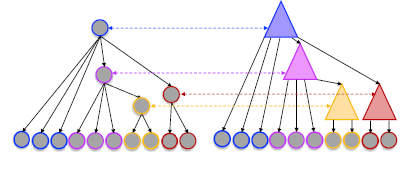
\includegraphics[width=14cm]{chaps/rw/scarlet_colon_tree}}
	\caption{مقایسه T’ از T}
	\label{fig:ch_rw:scarlet_colon_tree}
\end{figure}

مدل احتمالاتی برای توالی‌یابی داده:

\begin{figure}[!ht]
	\centerline{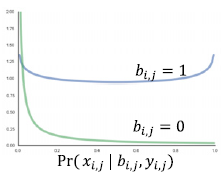
\includegraphics[width=9cm]{chaps/rw/scarlet_seq_model}}
	\caption{مدل احتمالاتی برای توالی‌یابی داده}
	\label{fig:ch_rw:scarlet_seq_model}
\end{figure}

ساختن درخت اتصالات T’ : 

\begin{figure}[!ht]
	\centerline{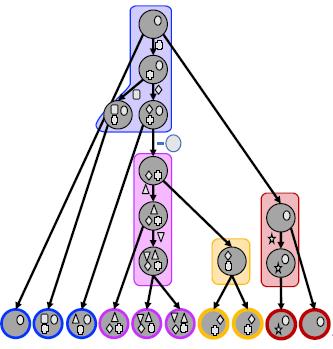
\includegraphics[width=9cm]{chaps/rw/scarlet_result}}
	\caption{ساختن درخت اتصالات T’}
	\label{fig:ch_rw:scarlet_result}
\end{figure}

و  در نهایت ماتریس جهش‌ها  \lr{B$^*$} با بیشینه \gls{likelihood}: 


\begin{figure}[!ht]
	\centerline{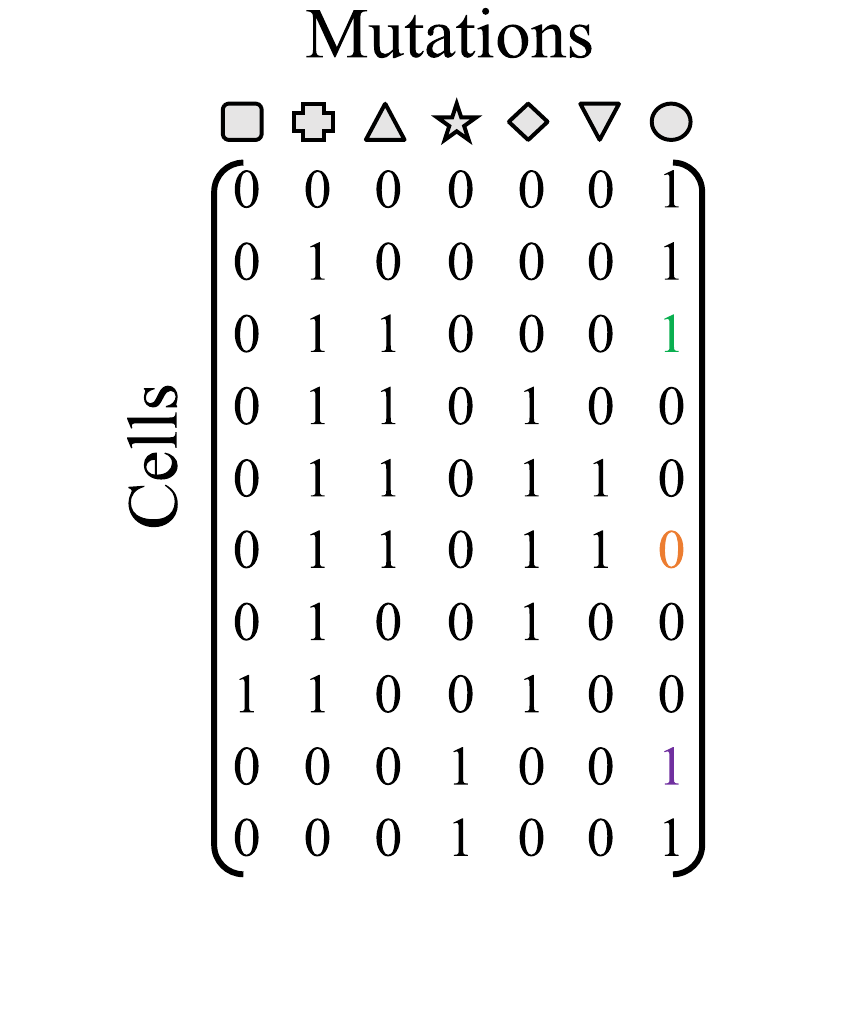
\includegraphics[width=4cm]{chaps/rw/scarlet_E}}
	\caption{ماتریس جهش‌ها \lr{B$^*$} با بیشینه \gls{likelihood}}
	\label{fig:ch_rw:scarlet_E}
\end{figure}


الگوریتم اسکارلت باید مسئله بیشینه \gls{likelihood} همراه با  انتخاب بهترین حذف‌ها را حل کند. این الگوریتم از طریق یافتن ماتریس جهش با بیشینه \gls{likelihood} \lr{B$^*$} انجام خواهد گرفت. در اینجا $L(T)$
مجموعه برگ‌های درخت \lr{T} را بیان می‌کند. 


\begin{math}
	y=xxxxxxxxxxxxxxxxxxx
\end{math}

الگوریتم اسکارلت از 2 قسمت اصلی زیر تشکیل شده است. 

\begin{itemize}
	\item      محاسبه وضعیت‌های جهش با بیشینه \gls{likelihood} \lr{R$^*$} از ریشه \gls{subtrees} 
	\item استنتاج هر زیردرخت به صورت مستقل با هدف بیشینه \gls{likelihood} با شرط داشتن \lr{R$^*$} .
\end{itemize}

در اینجا$I(T)$ مجموعه نودهای داخلی درخت \lr{T} را بیان می‌کند. 

\begin{math}
	y=xxxxxxxxxxxxxxxxxxx
\end{math}

مرحله اول:

\begin{math}
	y=xxxxxxxxxxxxxxxxxxx
\end{math}


در اینجا با فرض داشتن  \lr{R} راست نمایی محاسبه خواهد شد و  \lr{R$^*$}  با شمارش حالت جهش های معتبر برای هر موقعیت مکانی جهش a محاسبه شده و سپس بیشینه راست نمایی بالا حساب خواهد شد. 

مرحله دوم:  

یافتن \gls{subtrees} پایش‌شده: 

تعریف ماتریس سه‌تایی( \lr{ternary}) : مولفه‌های این ماتریس مقادیر 0 و 1 و ؟ می‌باشند.

\begin{math}
	y=xxxxxxxxxxxxxxxxxxx
\end{math}

و در نهایت حل معادله برنامه‌ریزی خطی عدد صحیح زیر: 

\begin{math}
	y=xxxxxxxxxxxxxxxxxxx
\end{math}


منوط به شروط زیر: 
\begin{math}
	y=xxxxxxxxxxxxxxxxxxx
\end{math}


با فرض اینکه \lr{M} عدد ثابت و بزرگی است: 

\begin{math}
	y=xxxxxxxxxxxxxxxxxxx
\end{math}


نقض \lr{$F_{w,a,b}$}
\begin{math}
	y=xxxxxxxxxxxxxxxxxxx
\end{math}


نقض \lr{$G_{w,a,b}$}

lr{$F_{w,a,b}$}
\begin{math}
	y=xxxxxxxxxxxxxxxxxxx
\end{math}


نقض \lr{$H_{w,a,b}$}

lr{$F_{w,a,b}$}
\begin{math}
	y=xxxxxxxxxxxxxxxxxxx
\end{math}


\section{الگوریتم \lr{DeepPhylo}  \cite{azer2020tumor}}

همانطور که می‌دانیم، سرطان یک بیماری تکاملی است که با تجمع تدریجی \gls{somaticmutation} در سلول های تومور مشخص می‌شود. رمزگشایی از تاریخچه تکاملی یک تومور، یک چالش مهم در مطالعات سرطان است و می تواند از جنبه‌های مهم بالینی از جمله \gls{tumorprogression}،  \gls{metastaticspread} و وجود \gls{divergentsubclones} در شاخه‌های مختلف درخت فیلوژنتیک تومور درک بهتری از تومور در اختیار ما بگذارد. با توجه به اهمیت مسئله، تحولات سریعی در طراحی روش‌های محاسباتی اصولی برای استنباط فیلوژنی تومور وجود داشته است.  بسیاری از این روش‌ها از \glspl{bulksequencingdata} استفاده می‌کنند که \lr{DNA} میلیون‌ها سلول سرطانی و طبیعی با هم یک توالی را تشکیل می‌دهند. استنباط درخت فیلوژنی با استفاده از این نوع داده‌ها، معمولاً بر مبنای \gls{detectedvariants} از بخش‌های مختلف سلول‌های سرطانی انجام می‌شود. به عنوان مثال:
 \gls{snv} \cite{strino2013trap, el2015reconstruction, malikic2020studying, donmez2016clonality, satas2017tumor, husic2019mipup}،  \gls{cnv} \cite{zaccaria2017copy}، \gls{structuralvariant} \cite{eaton2018deconvolution, ricketts2020meltos}.
 
 اگرچه استنباط درخت فیلوژنی با استفاده از این نوع داده مقرون به صرفه است اما \gls{resolution} پایین \glspl{bulksequencingdata} یک فاکتور محدود کننده در مدل‌سازی تکامل تومور است. به طور خاص \glspl{bulksequencingdata} ناشی از یک نمونه تومور به طور معمول یک توپولوژی خطی را به عنوان یک راه حل بهینه در تعیین درخت فیلوژنی تومور درنظر می‌گیرد. \cite{donmez2016clonality}
 
 
 با این حال، دانستن اینکه آیا تومور شامل زیرکلون‌های واگرایی است که از طریق شاخه‌های متمایزی از فیلوژنی تومور تکامل می‌یابند، گام مهمی در جهت درک بهتر پیشرفت تومور و بهبود طرح درمانی است. تحولات اخیر تکنولوژی، محققان را قادر به انجام آزمایش‌های \gls{scs} کرده است ، جایی که \lr{DNA} از یک سلول استخراج ، تکثیر و توالی‌یابی می‌شود. \gls{scs}، داده‌هایی با رزولوشن بالا برای مطالعه تکامل تومور با جزئیات زیاد را فراهم می‌کند، به عنوان مثال، امکان شناسایی توپولوژی شاخه‌ای با اطمینان بالا یا حل مشکل کلی استنباط کامل تاریخ تکامل تومور را فراهم می‌کند، حتی زمانی که تمام سلول‌های تک توالی که از یک نمونه \gls{biopsy} توموری استخراج شده باشد. روش‌های متعددی برای استنباط تاریحچه تکاملی تومور  از طریق  \gls{scs} وجود دارد که از مهمترین آنها می‌توان به موارد زیر اشاره کرد :  
 
 \begin{itemize}
 	\item رویکردهای مبتنی بر آمار و احتمالات که از فرض \gls{infinitesites}  استفاده می‌کنند. مثل الگوریتم \ lr{SCITE}  \cite{jahn2016tree} و الگوریتم  \lr{OncoNEM} \cite{ross2016onconem}. 
\item رویکردهایی که از فرض \gls{infinitesites} استفاده نمی‌کنند و فرض را بر این می‌گذارند که تخطی‌های در شکل‌گیری درخت تکاملی فیلوژنی تا یک مقدار خطا مشخص وجود دارد، مثل الگوریتم \lr{SiFit} \cite{zafar2017sifit}.  
 \end{itemize}


به تازگی الگوریتم‌هایی مثل \lr{SPhyR} که از یک رویکرد بهینه‌سازی ترکیبی مبتنی بر \gls{dolloparsimony} استفاده می‌کنند یا الگوریتم  \lr{SiCloneFit} که بهینه یافته الگوریتم \lr{SiFit} می‌باشد، ارائه شده است. \cite{el2018sphyr, zafar2019siclonefit}

شایان ذکر است که روش‌های همچون \lr{PhISCS-BnB} ، که از روش‌های بهینه‌سازی بر مبنای \gls{branchbound} استفاده می‌کنند، و یا روش‌هایی مثل \lr{ScisTree}، که بر مبنای \gls{joiningbasedheuristic} عمل می‌کند، به منظور بهبود زمان محاسباتی استنباط درخت فیلوژنی تومور ارائه شده‌اند. \cite{sadeqi2020phiscs, wu2020accurate}

در حالتی که هم \glspl{bulksequencingdata} و هم داده‌های \gls{scs} موجود باشد می‌توان تقریب دقیق‌تری از درخت فیلوژنی  تومور بدست آورد. \cite{malikic2019integrative, malikic2019phiscs}

همانطور که در بالا خلاصه شد، روش‌های موجود برای بازسازی فیلوژنی تومور با استفاده از داده‌های \gls{scs} محدودیت‌های مهمی دارند. اولاً ، بسیاری از این روش‌ها، فرض \gls{infinitesites} را به کار می‌گیرند (حتی در مواقعی که شرایطی برای \gls{limitedloss} و \gls{concordantgainofmutations}  در نظر گرفته شود) و سطح نویز یکنواختی را در نظر می‌گیرند (\gls{falsenegative} و همچنین نرخ \gls{falsepositive})  هر دو این محدودیت ها، با پیشرفت درک ما از تکامل تومور و فناوری \gls{scs}  تغییر می‌کند. مهمتر از همه ، هدف از این روش‌ها استنباط محتمل‌ترین درخت فیلوژنی توموری است و برای حذف نویز (به دلیل مثال ، \gls{alleledropout} یا \gls{lowsequencecoverage}) از روش‌های همچون \gls{maximumlikelihood} یا \gls{maximumparsimony} استفاده می‌کنند. به بیان دیگر این روش‌ها قصد دارند تا یک مساله پارامتری از مرتبه \lr{n} را حل کنند ولی بدلیل  عدم مقیاس‌بندی داده‌های \gls{scs} به مرتبه‌های بزرگتر، در حل دقیق این مساله ناتوان هستند. حتی وقتی هدف این است که به جای بازسازی کامل درخت فیلوژنی تومور، فقط ویژگی‌های اساسی توپولوژی فیلوژنی تومور را استنباط کنیم، این روش‌ها نمی‌توانند به راحتی داده‌های \gls{scs} شامل چند صد جهش و سلول را کنترل کنند. در نتیجه ، تکنیک‌های سریع برای استنباط ویژگی‌های کلیدی فیلوژنی تومور، به عنوان مثال، مواردی که می‌توانند توپولوژی‌های شاخه‌ای را از هم تفکیک کنند، به ویژه برای مجموعه داده‌های \gls{scs} با سطح نویز بالا از محبوبیت بیشتری برخوردار هستند. به همین منظور ، بهتر است در ابتدا به این سوال پاسخ داده شود که آیا حذف نویز  برای ساخت فیلوژنی کامل لازم است یا خیر. سرانجام، هر یک از ابزارهای موجود به تلاش انسانی زیادی در طراحی و اجرای الگوریتمی نیاز داشته است، زیرا هر پیشرفت تکنولوژیکی در تولید داده‌ها، توسعه روش‌های کاملاً جدید را ضروری می‌کند. بنابراین داشتن یک رویکرد محاسباتی کلی که بتواند با تغییر منطقی تکنیکی سازگار شود، صرفاً از طریق آموزش آن با دادههای جدید، بدون نیاز به مدل‌سازی صریح مشخصات نویز، بسیار مطلوب است.


رفع این محدودیت‌ها از طریق رویکرد یادگیری ماشینی یا رویکردهای "داده محور" امکان پذیر است که مجموعه‌ای کلی از توابع را در نظر گرفته و تابعی را در نهایت انتخاب می‌کند که برآورد بهتری از مجموعه داده‌های آموزشی (دادگان واقعی یا شبیه‌سازی شده) باشد. چنین رویکردی نه تنها می‌تواند از عدم دقت در مدل‌سازی مشخصات نویز بکاهد بلکه الگوهای اساسی ضمنی را در داده‌ها یا مسئله را برای توسعه اهداف واقع بینانه‌تر شناسایی می‌کند. پیشرفت‌های اخیر در \gls{deeplearning} تعمیم قابل توجهی از فرمول‌بندی‌ها را برای حل بسیاری از مشکلات نشان داده است. \cite{silver2017mastering, devlin2018bert, liu2019roberta}

این امکان وجود دارد که یک معماری یادگیری عمیق ، زمانی که بتواند در تعداد کافی مجموعه داده آموزش را دیده باشد، بتواند در استنباط خواص متمایز از فیلوژنی های تومور موفق شود.  در سالهای اخیر ، بسیاری از برنامه‌های محاسباتی، رویکرد الگوریتمی خود را به رویکردهای داده محور تغییر داده‌اند. مانند رمزگشایی متن دست نوشته برای شناسایی رقم \cite{ciregan2012multi} و پردازش زبان طبیعی. \cite{devlin2018bert}

مسائلی که در بایولوژی ساختار یافته، فرمول‌سازی هدفمند یا کمی‌سازی آنها مشکل است (مانند استنباط ساختار سه بعدی توالی پروتئینی) از روشهای مبتنی بر یادگیری عمیق بشترین استفاده را در جهت حل مسائل خواهند کرد. \cite{senior2020improved}

با این حال این مقاله، اولین مقاله استنباط درخت فیلوژنی تومور مبتنی بر رویکردهای داده محور است. در این مقاله، اولین روش‌های بازسازی فیلوژنی تومور مبتنی بر داده را برای رفع محدودیت‌های استراتژی‌های موجود ارائه شده است. نویسندگان این مقاله از داده‌های \gls{scs} در کنار شبکه‌های عصبی عمیق و یادگیری تقویتی برای استنباط ویژگی‌های توپولوژیکی فیلوژنی تومور و همچنین محتمل‌ترین سابقه تکاملی تومور استفاده شده‌است. برای رسیدن به  این هدف، چندین چالش وجود داشت: 

\begin{enumerate}
	\item     شبکه عصبی در حالت ایده‌آل باید طوری طراحی شود که بتواند تعداد متفاوتی از سلول‌ها و جهش‌ها را کنترل کند.  متناوباً، برای مدل‌هایی با ورودی‌هایی با اندازه ثابت‌، بهتر است که از دانش خود در زمینه تهیه داده استفاده شود تا داده‌ها به روشی تهیه شود تا موفقیت در پیش‌بینی‌ها را تسهیل کند. 
	\item با توجه به استفاده از شبکه‌های عصبی، برای آموزش مناسب به تعداد زیادی نمونه نیاز است. متأسفانه، تعداد مجموعه داده‌های \gls{scs} تومور در دسترس عموم برای آموزش مدل‌های یادگیری عمیق به اندازه کافی زیاد نیست. بنابراین، نیاز به تولید تعداد زیادی مجموعه داده شبیه‌سازی شده داده‌های \gls{scs} وجود دارد.  
	\item نویز و خطاهای موجود در داده های توالی یابی تک سلولی پیچیدگی بیشتری را به این مسئله می‌افزاید و چارچوب پیشنهادی یادگیری عمیق باید از نظر تحمل نویز  ارزیابی شود.  
	\item معماری انتخاب شده مستلزم نوع خاصی از نظارت است که ما باید قادر به تامین آن باشیم.
\end{enumerate}

به منظور کاهش یا حذف نویز در ورودی "ماتریس ژنوتیپ" استخراج شده از داده‌های \gls{scs}، می توان نظارت را به صورت مجموعه داده‌ای از ورودی‌های نویزدار به همراه با ورودی‌های بدون نویز ارائه داد. یک نظارت جایگزین و ارزان تر توسط مکانیزم \gls{feedback} است که تعیین می‌کند که آیا  یک خروجی  از شبکه عصبی با موفقیت بدون نویز شده است یا خیر. گزینه سوم توسط یک تابع هزینه ارائه می‌شود که به طور غیرمستقیم کمک به نظارت بر فرایند یادگیری تقویتی می‌کند. 

در این مقاله با الهام از رویکردهای جدید یادگیری عمیق  برای مسائل گوناگون مانند "الگوریتم گرادیان سیاست تقویتی" برای مساله فروشنده دوره گرد\cite{williams1992simple}،  رویکرد \lr{NeuroSAT} \cite{selsam2018learning} برای مساله رضایت‌مندی با استفاده از نظارت تک‌بیتی، یک چارچوب محاسباتی ایجاد شد تا همه چالش‌های فوق را به شرح زیر با موفقیت حل کند.
\begin{enumerate}
	\item     یک رویکرد مبتنی بر یادگیری تقویتی به منظور آموزش مدلی جهت از بین بردن نویز داده‌ها بدون نیاز به \gls{goldstandard} به کار گرفته شد. تابع هزینه استفاده شده در این مدل یک تابع هزینه خاص برای رفع مساله از بین بردن نویز بود. 
    
    \begin{math}
    	y=xxxxxxxxxxxxxxxxxxxxx
    \end{math}

که در آن \lr{X} ماتریس خروجی ناشی از ورودی A’ است. 
\item     داده‌های ماتریس ورودی، که از مجموعه دادگان نویزی \gls{scs} استخراج شده، در کنار نرخ نویز و موقعیت مکانی به عنوان ورودی به شبکه داده شده است.  این رویکرد در مجموعه دادگانی با سایز متفاوت همچنان کارآمد است و مستقل از جابجایی در سطر و ستون ماتریس ورودی است. 
\item یک مرحله پیش‌پردازش دیتا، به منظور به کارگیری دانش حاصل از تجربه در نظر گفته شده است تا هر گونه عملکردی را  که می‌تواند پیش‌بینی مدل را بهبود بخشد، بر روی داده‌ها اعمال گردد. 
\item داده‌های شبیه‌سازی شده ورودی مدل از طریق یک چاچوربی که راستی‌آزمایی شده است، توسعه یافته است. 
\end{enumerate}

در نمودار \ref{fig:ch_rw:deep_phylo_charts}، میزان دقت علمکرد شبکه در حذف نویز داده ورودی و تاثیر مرحله پیش‌پردازش بر خروجی الگوریتم را مشاهده می‌کنید. همچنین تاثیر میزان نرخ نویزی بودن داده‌ها در خروجی شبکه قابل توجه است. تصاویر \lr{A} و \lr{C} میزان دقت شبکه در حذف نویز داده‌هایی را نشان می‌دهد که با نزخ نویزهای  \lr{$\alpha = 0.02$} و \lr{$\beta = 0.1$} نمونه‌برداری شده‌اند اما  تصاویر \lr{B} و \lr{C} میزان دقت شبکه در حذف نویز داده‌هایی را نشان می‌دهد که با نرخ‌های کاذب مثبت \lr{$\alpha = 0.00004$} و کاذب منفی \lr{$\beta = 0.002$} نمونه‌برداری شده است.  


\begin{figure}[!ht]
	\centerline{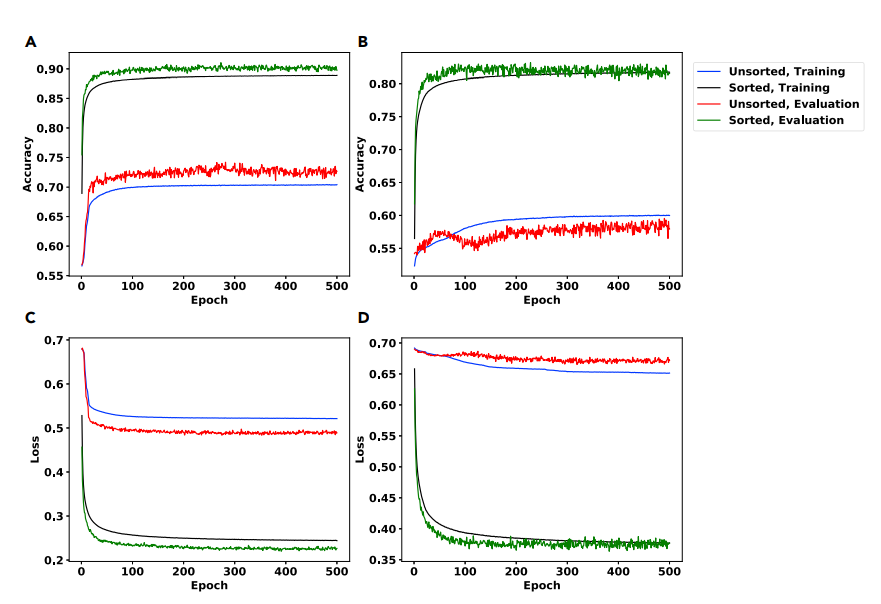
\includegraphics[width=15cm]{chaps/rw/deep_phylo_charts}}
	\caption{عععععععععععععععععععععععععععععععععععععععع}
	\label{fig:ch_rw:deep_phylo_charts}
\end{figure}

همچنین در جدول \ref{tab:table_55} تاثیر مرحله پیش‌پردازش دیتا در دقت خروجی مدل در حذف نویز از دیتا را مشاهده می‌کنید که میزان دقت حذف نویز بهبود قابل قبولی داشته است. 

\begin{latin}
\begin{table}[!ht]
	\centering
	\begin{tabular}{|c|c|c|c|c|}
		\hline
		\rowcolor[gray]{0.9}
		Input MAtrix Size & A            & B        & Unsorted Acc. & Sorted Acc.  	 \\\hline
		10*10               & $0.002$       & $0.1$    & 72            & 90          \\\hline
		10*10               & $4*10^{-4}$   & $0.02$   & 60            & 81          \\\hline
		25*25               & $3.2*10^{-4}$ & $0.016$  & 50            & 77          \\\hline
		25*25               & $6.4*10^{-4}$ & $0.0032$ & 52            & 65         \\\hline
	\end{tabular}\par
\caption{ffffffffffffffffffffffff}
\label{tab:table_55}
\end{table}
\end{latin}



در نهایت مقایسه بین عملکرد الگوریتم پیشنهادی در این مقاله و الگوریتم \lr{PhISCS} با استفاده از معیار شباهت \lr{MLTSM84} انجام شد که نتجیه این مقایسه در شکل \ref{fig:ch_rw:deep_phylo_mltsm} آمده است. همانطور که در شکل \ref{fig:ch_rw:deep_phylo_mltsm} مشهود است عملکرد الگوریتم پیشنهادی در میزان شباهت‌های مشابه، تعداد استنباط‌های بیشتری از فیلوژنی تومور را شامل می‌شود. 


\begin{figure}[!ht]
	\centerline{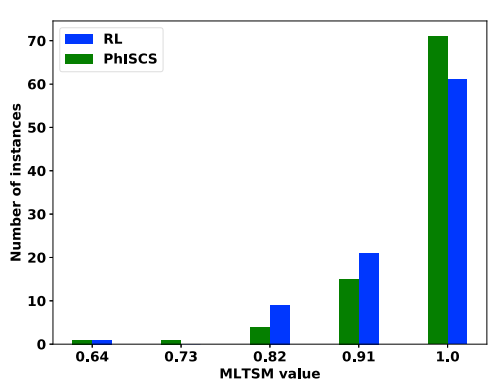
\includegraphics[width=9cm]{chaps/rw/deep_phylo_mltsm}}
	\caption{عععععععععععععععععععععععععععععععععععععععع}
	\label{fig:ch_rw:deep_phylo_mltsm}
\end{figure}


خلاصهای از سازکار به کار رفته در این مقاله در شکل \ref{fig:ch_rw:deep_phylo} آمده است: 

\begin{figure}[!ht]
	\centerline{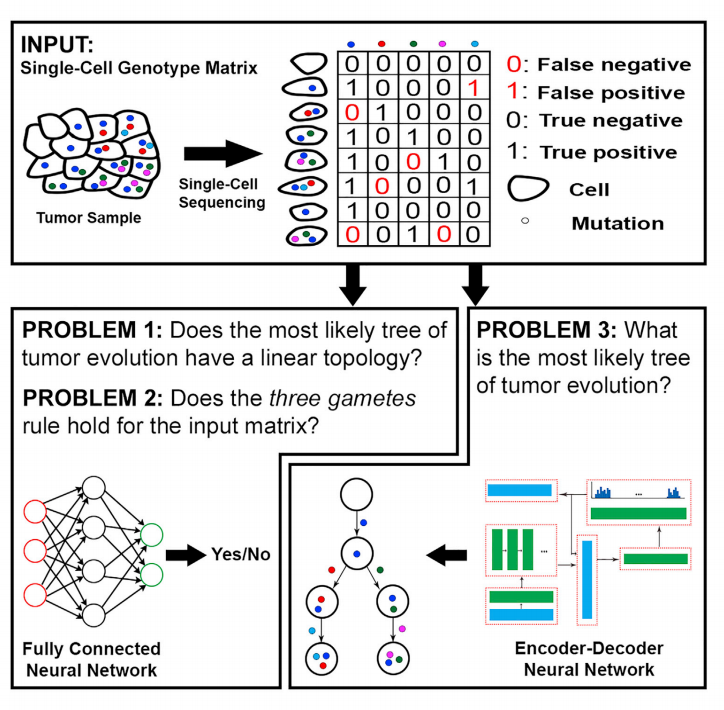
\includegraphics[width=12cm]{chaps/rw/deep_phylo}}
	\caption{عععععععععععععععععععععععععععععععععععععععع}
	\label{fig:ch_rw:deep_phylo}
\end{figure}





\section{جمع‌بندی}

جهش‌های سومایتک تومورها در تمام مقیاس‌های ژنومی، از  \glspl{snvv} (\lr{SNV}) تا جهش‌های \gls{cnv} (\lr{CNA}) وجود دارد. تا به امروز ، بیشتر روش‌های ساخت فیلوژنی توموری از داده های \gls{scs} \lr{DNA} فقط از  \glspl{snvv} استفاده می‌کردند.  \cite{singer2018single, malikic2015clonality, mcpherson2016divergent, el2018sphyr}  و جهش‌های \gls{cnv} و در نتیجه اطلاعات مهم استنباط فیلوژنیک تومور را نادیده می‌گرفتند. 


وجود ناهمگنی‌های درون توموری باعث ناکارآمدی درمان‌های دارویی تومور می‌شود زیرا که هر یک از این روش‌های درمانی به طور موثر فقط بر روی تعداد محدودی از کلون‌های توموری اثر می‌گذارند و همه این زیرنواحی را تحت تاثیر قرار نمی‌دهند. با مطالعه بر روی تومورهای مختلف این امکان حاصل می‌شود تا الگوهای درون توموری بهتر شناخته شوند و درمان داریی تومور کارآمدتر و بهینه‌تر از گذشته صورت بپذیرد. مطالعه بر روی داده‌های \gls{scs} یکی از زمینه‌های تحقیقاتی است که می‌تواند منجر به افزایش دانش از نحوه شکل‌گیری و تکامل تومور شود. پیدا کردن سیر زمانی تکامل تومور با استفاده از داده‌های \gls{scs} چالشی است که اخیراً مورد توجه قرار گرفته است که در جدول زیر خلاصه‌ای از روش‌هایی که در این فصل مورد بررسی قرار گرفته‌اند، مشاهده می‌شود. 

\begin{sidewaystable}
	\caption{Comparison}
	\begin{latin}
		\centering
	    \tiny
		\begin{tabular}{|p{0.1\textheight}|p{0.14\textheight}|p{0.1\textheight}|p{0.1\textheight}|p{0.14\textheight}|p{0.14\textheight}|}
			\hline
			\rowcolor[gray]{0.9}
			Method & Dataset & Algorithm & Output & Evaluation Method & Limitation \\\hline
			% Row 1
			Kim \& Simon approach &
			Thrombocythemia Essental (TE) &			
			Minimal spanning tree of the Edmonds’ algorithm &		
			Phylogenic tree &	
			Leave one out cross validation &
			high computational time and excluding uncertainty dataset error \\\hline
			% Row 2
			BitPhylogeny &
			JAK2 negative myloprolifirative &
			TSSB, MCMC &
			Evolutionary clonal tree &
			$V$ measure comparison with K-Centroids  and Hierarchical Clustering &
			High computational time, infinte sites assumption and homozigot-heterozigot differentiation \\\hline
			% Row 3
			SCITE &
			JAK2 negative myloprolifirative, clear cell and  renal cell carcinoma, estrogen-receptor positive breast cancer  &
			Maximum liklihood, bayesian MCMC &
			Phylogenic tree &
			Better performance in real dataset in comparison with bitphylogeny algorithm &
			Infinte sites assumption \\\hline
			% Row 4
			ONCONEM &
			Muscle invasive bladder transitional cell carcinoma &
			Neighbor joining, MCMC &
			Phylogenic tree,evolutionary clonal tree &
			Score funtion extracted from nested model &
			infinte sites assumption, homozigot-heterozigot differentiation \\\hline
			% Row 5
			SASC &
			Muscle invasive bladder transitional cell carcinoma,Thrombocythemia Essental (TE)  
			Robust approach based on &
			Simulated annealing &
			Phylogenic tree &
			Better performance in real dataset in comparison with SCITE algorithm &
			Limited mutation assumption \\\hline
			% Row 6
			SCARLET &
			scDNA-seq data from a metastatic colorectal cancer patient &
			Loss-Supported Phylogeny Model &
			Phylogenic tree &
			Mutation matrix error and pairwise ancestral relationship error &
			Mutation loss due to the dollo assumption \\\hline
			% Row 7
			DeepPhylo &
			Acute Lymphoblastic Leukemia, TNBC dataset &
			Critic-actor reinforcement learning &
			Phylogenetic tree &
			Accuracy, maximum likelihood &
			Fixed input dimension, lack of empirical experiment \\\hline
		\end{tabular}
	\end{latin}
	\label{tab:ch_rw:comp_methods}
\end{sidewaystable}
